\documentclass[11pt, twoside, colorbacktitle, accentcolor=tud1b, nopartpage, bigchapter,
 fleqn, ngerman, longdoc]{tudreport}
%\documentclass[11pt, a4paper, twoside, fleqn, ngerman]{scrreprt}
% =================================================================================
% Falls scrreprt anstelle von tudreport gewählt, muss das über diesen Schalter
% mitgeteilt werden!
% =================================================================================
\newif\ifStdClassDraft
\StdClassDraftfalse	% tudreport
%\StdClassDrafttrue		% scrreprt



\makeatletter
\DeclareOldFontCommand{\sc}{\normalfont\scshape}{\@nomath\sc}
\makeatother


% =================================================================================

% =================================================================================
% Hier Daten für studentische Arbeit eingeben
% =================================================================================
% Wenn studentische Arbeit, müssen hier für Titel, Seite nach Titel und Erklärung
% einige Angaben gemacht werden:
\newcommand{\SADATyp}{Master-Thesis}
\newcommand{\SADATitel}{Modellierung und Regelung einer mechanischen Presse mithilfe von Methoden des maschinellen Lernens}
\newcommand{\SADAStadt}{Darmstadt}
\newcommand{\SADAAutor}{Tajinder Singh Dhaliwal}
\newcommand{\SADAAutorII}{}
\newcommand{\SADABetreuer}{Florian Hoppe}
\newcommand{\SADABetreuerII}{}
\newcommand{\SADABetreuerIII}{}
\newcommand{\SADABegin}{27. April 2015}
\newcommand{\SADAAbgabe}{28. April 2015}
\newcommand{\SADASeminar}{29. April 2015}

% Die folgende Zeile deklariert die möglichen Varianten der Erklärung, dass die
% Arbeit ohne Hilfe Dritter etc. erstellt wurde.
\def\MBMA{MBMA}\def\MBDA{MBDA}
% Es ist eine der möglichen Varianten auszuwählen:
%	MBDA	Für Maschinenbauer, Diplomarbeiten
%	MBMA	Für Maschinenbauer, Standard für Projektseminare und Abschlussarbeiten
% Entsprechende Zeile einkommentieren
\def\SADAVarianteErklaerung{MBMA}
%\def\SADAVarianteErklaerung{MBDA}
% =================================================================================


% =================================================================================
% Hauptdefintionen sind aus Platzgründen ausgelagert
% =================================================================================
% Einbinden wichtiger und weniger wichtiger Pakete

% Dieses File dient zum einbinden wichtiger und n�tzlicher Pakete.
% Nicht alle Pakete m�ssen verwendet werden.
%
\usepackage{etex}
\reserveinserts{28}
\usepackage{pdfpages} 
\usepackage{t1enc}			% evtl. dc-Fonts
\usepackage[T1]{fontenc}	% F�r Silbentrennung bei W�rten mit Sonderzeichen (z.B. Umlaute)
\usepackage[utf8]{inputenc}
							% Um Sonderzeichen (�, �, �, ...) direkt eingeben zu k�nnen
\usepackage[english,ngerman]{babel}
							% F�r Sprachenspezifisches
							% ngerman ist schon als globale Option definiert

%\usepackage{helvet}			% Helvetica als Standard-Sans-Schriftart
\usepackage[stable]{footmisc}
\usepackage{booktabs}
\usepackage{adjustbox}

\usepackage{graphicx}		% zum Einbinden von Postscript
\usepackage{psfrag}			% Beschriftung der Bilder
\usepackage{amsmath}		% Mehr mathematischen Formelsatz
\usepackage{sistyle}                            % für korrekten Abstand zwischen zahl und einheit, sowie aufrecht geschriebenen einheiten Bsp.: \SI{10}{mm}
%\usepackage{amssymb}		% Mehr mathematische Symbole
%\usepackage{amsthm}

\usepackage{float}			% F�r Parameter [H] bei Flie�objekten
\usepackage{dsfont}			% Befehleh f�r nat�rliche Zahlen R, Z 

\usepackage{subfigure}      	% F�r Unterabbildungen NEU Neu NeuNeu Neu Neu Neu Neu

\usepackage{epsfig}			% Um eps-Bilder einzubinden
%\usepackage{subfig}			% F�r Unterabbildungen
\usepackage{ltxtable} 		% Vereinigt TabularX und Longtable
\usepackage{rotating}		% Zum Drehen von Objekten
\usepackage{bibgerm}		% F�r deutsche Literaturverwaltung
%\usepackage{wrapfig}		% F�r kleine Bilder am Rand
%\usepackage{floatflt}		% Alternative zu wrapfig
%\usepackage[hang]{caption}	% Damit mehrzeilige Bildunterschriften gut aussehen
\usepackage{upgreek}		% F�r nicht-kursive kleine griechischen Buchstaben

\usepackage{multirow}		% F�r mehrzeilige Felder in Tabellen

\usepackage{textcomp}		% F�r Sonderzeichen im normalen Text
							% (offensichtlich in tudreport schon eingebunden)
\usepackage[ngerman]{varioref}		% F�r vref
\usepackage{color}			% F�r farbigen Text
\usepackage{placeins}		% F�r \FloatBarrier
\usepackage{xspace}
\usepackage{icomma}			% Damit nach Dezimalkommas kein Abstand eingef�gt wird
							% (in math-Umgebungen)

\usepackage{cancel}			% Zum Wegstreichen von Gleichungstermen

\usepackage{array}			% F�r Zellentyp "m{}" in tabular-Umgebungen (Vertikal zentriert)

\usepackage{listings}		% Um formatierten Quellcode einzubinden
\usepackage{moreverb}		% F�r Umgebung "`verbatimtab"' (Verbatim mit Tabs)
\renewcommand{\verbatimtabsize}{4\relax}	% Standardtabweite in "`verbatimtab"'
											% ist 4 Zeichen
%\usepackage{timing}
% Das Packet hyperref immer als letztes einbinden!
%\usepackage[ps2pdf, colorlinks=false, pdfborder={0 0 0}]{hyperref}
%\usepackage[ps2pdf, breaklinks=true]{hyperref}	% F�r Verlinkungen im erzeugten pdf
\usepackage[breaklinks=true]{hyperref}

% Seit 01.04.2018 eine digitale Version auf tabuma im PDF/A Dokument eingereicht werden.
\usepackage[a-1b]{pdfx}

%Tikz-Hilfen und PGF-Plots einbinden  
\usepackage{tikz}

\usetikzlibrary{arrows,calc}
\usetikzlibrary{positioning}
\usetikzlibrary{shapes}
\usetikzlibrary{backgrounds}
\usetikzlibrary{patterns}
\usetikzlibrary{fit}
\usetikzlibrary{decorations.markings}

\usepackage{pgfplots}


\newcommand{\TikZscale}{1}
\newcommand{\mm}{*\TikZscale mm}
% \input{d:/TikZ/TikZ_BSBnormal}

% TikZstyles f�r Blockschaltbilder
\tikzset{every picture/.style={auto, node distance=5\mm, >=stealth'}}

%% Bl�cke
	% Rechteckige Bl�cke
	\tikzstyle{blockS}     = [draw, rectangle, minimum height=15\mm, minimum width=30\mm, inner sep=3pt]
	\tikzstyle{NLblockS}   = [draw, rectangle, minimum height=15\mm, minimum width=30\mm, inner sep=3pt, double distance=4pt]	
	\tikzstyle{Trans}     = [draw, rectangle, minimum height=2\mm, minimum width=9\mm, inner sep=3pt]	
	
	\tikzstyle{block}      = [draw, rectangle, minimum height=10\mm, minimum width=10\mm, inner sep=3pt]
	\tikzstyle{NLblock}    = [draw, rectangle, minimum height=10\mm, minimum width=10\mm, inner sep=3pt, double distance=1.2pt]
	\tikzstyle{PICblock}   = [draw, rectangle, minimum height=10\mm, minimum width=10\mm, inner sep=2pt]
	\tikzstyle{NLPICblock} = [draw, rectangle, minimum height=10\mm, minimum width=10\mm, inner sep=3pt, double distance=1.2pt]
	\tikzstyle{noblock}		 = [rectangle, inner sep=-0.6pt]
	\tikzstyle{port}			=[draw, rectangle, minimum height=4\mm, minimum width=7\mm,rounded corners=2\mm]

	% Dreieckige Bl�cke
	\tikzstyle{Rgain}			 = [draw, isosceles triangle, inner sep=1pt, minimum width=13\mm, isosceles triangle apex angle=43]
	\tikzstyle{Lgain}			 = [draw, isosceles triangle, inner sep=1pt, minimum height=9\mm, isosceles triangle apex angle=60, shape border rotate=180]
	\tikzstyle{Ugain}			 = [draw, isosceles triangle, inner sep=1pt, minimum height=9\mm, isosceles triangle apex angle=60, shape border rotate=90]
	\tikzstyle{Dgain}			 = [draw, isosceles triangle, inner sep=1pt, minimum height=9\mm, isosceles triangle apex angle=60, shape border rotate=-90]

	% Runde Bl�cke
	\tikzstyle{sum}   	   = [draw, circle, inner sep=1pt, minimum size=3\mm]
	\tikzstyle{branch}		 = [draw, circle, inner sep=0pt, minimum size=1\mm, fill=black]


%% Verbindungselemente
	% Linien mit Pfeil
	\tikzstyle{bo}		=[dashed, thin]
	\tikzstyle{to}  		= [->, thick]
	\tikzstyle{toNL}		= [->, thick, shorten >=0.6pt]
	\tikzstyle{NLto}		= [->, thick, shorten <=0.6pt]
	\tikzstyle{NLtoNL}	= [->, thick, shorten <=0.6pt, shorten >=0.6pt]
	
	% Doppellinien mit Pfeil
	\tikzstyle{TO}  		= [semithick, double distance=2pt, shorten >=2mm, decoration={markings,mark=at position 1 with {\arrow[semithick]{open triangle 60}}}, postaction={decorate}]
	
	\tikzstyle{TONL} = [semithick, double distance=2pt, shorten >=2.2mm, decoration={markings,mark=at position 1 with {\arrow[semithick]{open triangle 60}}, transform={xshift=-0.7pt}}, postaction={decorate}]
	
	\tikzstyle{NLTO} = [semithick, double distance=2pt, shorten <=0.79pt, shorten >=2mm, decoration={markings,mark=at position 1 with {\arrow[semithick]{open triangle 60}}}, postaction={decorate}]
	
	\tikzstyle{NLTONL} = [semithick, double distance=2pt, shorten <=0.79pt, shorten >=2.2mm, decoration={markings,mark=at position 1 with {\arrow[semithick]{open triangle 60}}, transform={xshift=-0.7pt}}, postaction={decorate}]
	

	% Linien ohne Pfeil 
	\tikzstyle{line}       = [thick]
	\tikzstyle{lineNL}     = [thick, shorten >= 0.6pt]
	\tikzstyle{NLline}     = [thick, shorten <= 2pt]
	\tikzstyle{NLlineNL}	 = [thick, shorten <= 0.6pt, shorten >= 0.6pt]
	\tikzstyle{LineBS}	 = [line width=0.6mm]

	
	% Doppellinien ohne Pfeil
	\tikzstyle{LINE}       = [semithick, double distance=2pt]
	\tikzstyle{LINENL}     = [semithick, double distance=2pt, shorten >= 0.6pt]
	\tikzstyle{NLLINE}     = [semithick, double distance=2pt, shorten <= 0.6pt]
	\tikzstyle{NLLINENL}	 = [semithick, double distance=2pt, shorten <= 0.6pt, shorten >= 0.6pt]
	
	
	% Pins und Labels
	\tikzstyle{every pin edge}	= [<-, thick]
	\tikzstyle{every pin}	 			= [pin distance=5\mm]
	\tikzstyle{every label}			= [font=\small, label distance=-2pt]
	\tikzstyle{terminal}				= [coordinate]




\newcommand{\mywidth}{40mm}
\newcommand{\myheight}{25mm}
%% Bilder f�r PICblock

%\newcommand{\TikZIntegrator}{
%\begin{tikzpicture}
	% Koordinatensystem
%	\draw[thin] (-7\mm,-5\mm) -- (7\mm,5\mm);
%\end{tikzpicture}


\newcommand{\TikZGain}{
\begin{tikzpicture}
		\draw (0,5\mm) -- (14\mm,5\mm);
		\draw[white] (0,0) -- (14\mm,0);
\end{tikzpicture}
}

\newcommand{\TikZsgn}{
\begin{tikzpicture}
	% Koordinatensystem
	\draw[->, very thin] (-4\mm,0) -- (4\mm,0);
	\draw[->, very thin] (0,-4\mm) -- (0,4\mm);
	
	% Signumfunktion
	\draw[thin] (-4\mm,-2\mm) -- (0,-2\mm);
	\draw[thin] (0,-2\mm) -- (0,2\mm);
	\draw[thin] (0,2\mm) -- (4\mm,2\mm);
\end{tikzpicture}
}

\newcommand{\TikZdeadzone}{
\begin{tikzpicture}
	% Koordinatensystem
	\draw[->, very thin] (-4\mm,0) -- (4\mm,0);
	\draw[->, very thin] (0,-4\mm) -- (0,4\mm);
	
	% Deadzone
	\draw[thin] (-3\mm,-4\mm) -- (-2\mm,0);
	\draw[thin] (-2\mm,0) -- (2\mm,0);
	\draw[thin] (2\mm,0) -- (3\mm,4\mm);
\end{tikzpicture}
}

\newcommand{\TikZsaturation}{
\begin{tikzpicture}
	% Koordinatensystem
	\draw[->, very thin] (-4\mm,0) -- (4\mm,0);
	\draw[->, very thin] (0,-4\mm) -- (0,4\mm);

	% Saturation
	\draw[thin] (-4\mm,-2.5\mm) -- (-1\mm,-2.5\mm);
	\draw[thin] (-1\mm,-2.5\mm) -- ( 1\mm, 2.5\mm);
	\draw[thin] ( 1\mm, 2.5\mm) -- ( 4\mm, 2.5\mm);
\end{tikzpicture}
}

%% sonstige Bilder
\newcommand{\TikZRarrow}[1][]{%
\begin{tikzpicture}
	\draw[<-,opacity=0] (-3.8\mm,0) -- (0,0) node[pos=0, anchor=south east, xshift=2\mm, yshift=1\mm] {#1};	% keine Ahnung warum, aber nur mit -3.8 wirds mittig....
	\draw[|->] (0,0) --  node[pos=1, anchor=south west, xshift=-2\mm, yshift=1\mm] {#1} (5\mm,0);
\end{tikzpicture}%
}

\newcommand{\TikZspring}[1][10]{%
\begin{tikzpicture}
	\foreach \x in{0,1,...,3}
		\draw[thick, line join=round, line cap=round] (#1*0.25*\x\mm,0) -- (#1*0.0625\mm+#1*0.25*\x\mm,2\mm) -- (#1*0.1875\mm+#1*0.25*\x\mm,-2\mm) -- (#1*0.25\mm+#1*0.25*\x\mm,0\mm);
	\draw[thick] (0,0) -- ++(-1\mm,0);
	\draw[thick] (#1\mm,0) -- ++(1\mm,0);
\end{tikzpicture}%
}

\newcommand{\TikZdamper}{%
\begin{tikzpicture}
	\draw[thick] (0,0) -- (2\mm,0);
	\draw[thick] (2\mm,1\mm) -- (2\mm,-1\mm);
	\draw[thick] (1\mm,1.5\mm) -- (3\mm,1.5\mm) -- (3\mm,-1.5\mm) -- (1\mm,-1.5\mm);
	\draw[thick] (3\mm,0) -- (5\mm,0);
\end{tikzpicture}%
}


\newcommand{\TikZrwall}{%
\begin{tikzpicture}
\draw[thick] (0,0\mm) -- (0,6\mm);
\draw[white] (0,0\mm) -- (0,-2\mm); % Damit der Block zentriert ist (unsch�ne L�sung...)
\foreach \x in{0,1,...,6}
	\draw (0,\x\mm) -- ++(2\mm,2\mm);
\end{tikzpicture}%
}

\newcommand{\TikZlwall}{%
\begin{tikzpicture}
	\draw[thick] (0,-0.2\mm) -- (0,4.1\mm);
	\foreach \x in{0,1,...,4}
		\draw (0,\x\mm) -- ++(-1.2\mm,-1.2\mm);
	\draw[opacity=0] (0,4.1\mm) -- (0,5.1\mm); % Damit der Block zentriert ist (unsch�ne L�sung...)
\end{tikzpicture}%
}
\pgfplotsset{/pgf/number format/use comma}

\newcommand{\xmin}{1e-2}
\newcommand{\xmax}{1e2}

\newcommand{\omegaD}{1}

\newcommand{\bodestyle}{
\pgfplotsset{ major grid style={line width=0.3pt, color=gray},
							minor grid style={line width=0.3pt, color=gray},
							major tick style={line width=0.4pt, color=black},
							major tick length={4pt},
							minor tick length={0pt},
							tick label style={font=\small}}
}

\newcommand{\nyquiststyle}{
\pgfplotsset{ major grid style={line width=0.3pt, color=gray},
							minor grid style={line width=0.3pt, color=gray},
							major tick style={line width=0.4pt, color=black},
							major tick length={4pt},
							minor tick length={0pt},
							tick label style={font=\small}}
}

\newcommand{\plotstyle}{
\pgfplotsset{ major grid style={line width=0.3pt, color=gray},
							minor grid style={line width=0.3pt, color=gray},
							major tick style={line width=0.4pt, color=black},
							major tick length={4pt},
							minor tick length={0pt},
							tick label style={font=\small}}
}


\newcommand{\plotyystyle}{
\pgfplotsset{every non boxed y axis/.style={ytick align=inside,y axis line style={-}},
						 every boxed y axis/.style={}}
}


\newenvironment{bodeAmpDB}[1][]{
\bodestyle
\begin{semilogxaxis}[	ylabel=$|G(\mathrm{j}\omega)|_{\mathrm{dB}}$,
											%ylabel=Amplitude in dB,
											ylabel style={yshift=2pt},
											xminorgrids=true, xmajorgrids=true,
		  								ymajorgrids=true, yminorgrids=true,
			  							xticklabels=\empty,
											width=\mywidth,
											height=\myheight,#1]
}{\end{semilogxaxis}}


\newenvironment{bodeAmpLOG}[1][]{
\begin{loglogaxis}[	ylabel=$|G(\mathrm{j}\omega)|$,
										ylabel=Amplitude,
										ylabel style={yshift=2pt},
										xminorgrids=true, xmajorgrids=true,
		  							ymajorgrids=true, yminorgrids=true,
			  						xticklabels=\empty,
										y tick label style={font=\small},
										width=\mywidth,
										height=\myheight,#1]
}{\end{loglogaxis}}


\newenvironment{bodePhase}[1][]{
\begin{scope}[yshift=-\myheight+12mm]	% zweiten Plot (Phase) unter den Amplitudengang setzen
	\bodestyle
	\begin{semilogxaxis}[xlabel=Frequenz $\omega$ in\ensuremath{\mathrm{{\frac{rad}{s}}}},
										   %ylabel=Phase in $^\circ$,
											 ylabel=$\angle{G(\mathrm{j}\omega)}$,
										   ylabel style={yshift=2pt},
											 xminorgrids=true, xmajorgrids=true,
		  								 ymajorgrids=true, yminorgrids=true,
											 ytick={-360, -315,..., 360},
											 yticklabel={$\pgfmathprintnumber{\tick}^\circ$}, % ° als Einheitenzeichen an alle yticks
										   width=\mywidth,
										   height=\myheight,#1]
}{\end{semilogxaxis}\end{scope}}


\newenvironment{plotyyLeft}[1][]{
\plotyystyle
\begin{axis}[scale only axis,
						 enlarge x limits=0,
						 axis y line=left,
						 width  = \mywidth,
						 height = \myheight,
						 #1]
}{\end{axis}}

\newenvironment{plotyyRight}[1][]{
\plotyystyle
\begin{axis}[scale only axis,
						 enlarge x limits=0,
						 axis y line=right,
						 axis x line=none,
						 width=\mywidth,
						 height=\myheight,
						 #1]
}{\end{axis}}

% Wichtige Einstellungen, immer verwenden!
% Dieses File dient f�r wichtige Einstellungen. �nderungen sind zu vermeiden.
%

% =================================================================================
% Anpassung Absatzformat
% =================================================================================
% Der Abstand der Zeilen betr�gt das 1,25-fache des Standard-Abstands von
% LaTeX. Da technische Arbeiten viele Formeln und Bilder enthalten, werden
% Abs�tze durch einen zus�tzlichen vertikalen Zwischenraum statt durch einen
% Einzug getrennt.
\linespread{1.25}
\setlength{\parindent}{0mm}
\setlength{\parskip}{1ex}

% =================================================================================

% =================================================================================
% Definitionen aus tudreport-Vorlage 
% =================================================================================

\newlength{\longtablewidth}
\setlength{\longtablewidth}{0.7\linewidth}
\addtolength{\longtablewidth}{-\marginparsep}
\addtolength{\longtablewidth}{-\marginparwidth}
% =================================================================================

% =================================================================================
% Farbige Deckseite, graue Balken auf allen anderen Seiten
% =================================================================================
\newif\ifOnlyColorFront
\OnlyColorFronttrue	% Balken nur auf Deckblatt farbig
%\OnlyColorFrontfalse		% alle Balken farbig

% =================================================================================
% Texte f�r den Titel und die R�ckseite des Titels vorgeben
% =================================================================================
\title{\SADATitel}
\subtitle{\SADAAutor}
\ifStdClassDraft
%
\else
    \subsubtitle{\SADATyp\ \SADAAbgabe  \\Betreuer: \SADABetreuer{} \SADABetreuerII{} \SADABetreuerIII{}}
% \settitlepicture{}	% Bild f�r Deckblatt
% \printpicturesize

        \newcommand{\SADAProf}{Prof. Dr.-Ing. Dipl.-Wirtsch.-Ing. Peter Groche}
        \newcommand{\SADAinstitut}{Institut f�r Produktionstechnik und Umformmaschinen\\
                                   \SADAProf}
        \newcommand{\SADAwebsite}{www.ptu.tu-darmstadt.de}
        \newcommand{\SADAtel}{06151/16-3056}
        \newcommand{\SADAlogo}{\includegraphics[width=3cm]{./common/PtU_Logo.eps}}

    \setinstitutionlogo[height]{common/PtU_Logo.eps}

\fi
% Folgende Eintr�ge werden auf der R�ckseite der Titelseite gedruckt:
\uppertitleback{}
\lowertitleback{}
\dedication{}
% =================================================================================

% =================================================================================
% Befehle, die in scrreprt nicht exisiteren werden hier definiert, wenn diese
% Klasse verwendet wird.
% Auch die Seitenr�nder werden angepasst, so dass es grob wie mit tudreport
% aussieht.
% =================================================================================
\ifStdClassDraft
    % Diese Pakete nur extra einbinden, wenn NICHT tudreport als Basis.
	\usepackage{amssymb}
	\usepackage{geometry}
	\newcommand{\subsubtitle}[1]{}
	\newcommand{\settitlepicture}[1]{}
	\newcommand{\printpicturesize}{}
	\newcommand{\institution}[1]{}
    \pagestyle{headings}
	
	\author{\SADAAutor}	% scrreprt erwartet Autor
\fi
% =================================================================================


% =================================================================================
% Informationen (Meta-Daten) f�r pdf
% =================================================================================
\hypersetup{
	pdftitle = {\SADATitel},
	pdfsubject = {},
	pdfauthor = {\SADAAutor},
	pdfkeywords = {},
	pdfcreator = {},
	pdfproducer = {LaTeX with hyperref},
	pdfstartview = {Fit},
	pdfpagelayout = {SinglePage}
}
% =================================================================================

% =================================================================================
% Anpassung der Seitenr�nder
% =================================================================================
% f�r bessere Lesbarkeit nach der Bindung
\geometry{left=30mm, right=20mm, top=15mm, bottom=20mm}
% ================================================================================= 

% Nützliche Befehle und Abkürzungen
% Dieses File dient zum definieren n�tzlicher Befehle.
% Es soll lediglich als Beispiel dienen, wie Befehle definiert werden, und welche Befehle n�tzlich sein k�nnen
%

% Spezielle Abk�rzungen - Projektseminar Hochregal
	\newcommand{\inch}{\textquotedbl{} }	% Zollzeichen mit anschlie�endem Leerzeichen
	\newcommand{\schneider}{\textsc{Schneider Electric}\@\xspace}
	
% Masterarbeit
	%Symbole
	\newcommand{\xmess}{x_{\mathrm{m}}}
	\newcommand{\wmess}{w_{\mathrm{m}}}
	\newcommand{\Fmess}{F_{\mathrm{m}}}
	\newcommand{\Erw}[1]{\mrm{E}[#1]}
	\newcommand{\varw}{\sigma^2_\mrm{w}}
	\newcommand{\varnu}{\sigma^2_\mrm{\nu}}
	\newcommand{\Iy}{I_\mrm{y}}
	\newcommand{\Iyl}{I_\mrm{yl}}
	\newcommand{\Iyh}{I_\mrm{yh}}
	\newcommand{\My}{M_\mrm{y}}
	\newcommand{\wU}{w_\mathrm{U}}
	\newcommand{\khat}{\hat{k}}
	\newcommand{\khatel}{\hat{k}_\mrm{el}}
	\newcommand{\khatpl}{\hat{k}_\mrm{pl}}
	\newcommand{\khatelm}{\hat{k}_{\mrm{el},m}}
	\newcommand{\kel}{k_\mrm{el}}
	\newcommand{\wO}{\bar{w}}
	\newcommand{\wOhat}{\tilde{w}}
	\newcommand{\wOsoll}{\wO_\mrm{soll}}
	\newcommand{\FY}{F_\mrm{Y}}
	\newcommand{\veFhat}{\hat{\ve{F}}}
	\newcommand{\vewhat}{\hat{\ve{w}}}
	\newcommand{\sY}{\sigma_\mrm{Y}}
	\newcommand{\sF}{\sigma_\mrm{F}}
	\newcommand{\that}{\hat{\ves{\theta}}}
	\newcommand{\BSigma}{\ves{\Sigma}}
	\newcommand{\Bmu}{\ves{\mu}}
	\newcommand{\Tabt}{T_\mrm{abt}}
	\newcommand{\ufrac}[2]{\frac{\mrm{#1}}{\mrm{#2}}}
	\newcommand{\delFw}{\frac{\Delta F}{\Delta w}}
%	\newcommand{\argmin}{
	% Befehle
	\newcommand{\mtrx}[1]{\begin{bmatrix}#1\end{bmatrix}}
	\newcommand{\partialdd}[2] { \frac{\partial^2 #1 }{\partial #2 ^2 } }
	\newcommand{\normdd}[2] { \frac{\mathrm{d}^2 #1 }{\mathrm{d} #2 ^2 } }
	
	
% Inhalt
% ======
%	Allgemeine Abk�rzungen
%	Makros f�r Referenzen (Abbildungen, Zitate, ...)
%	Makros f�r Abbildungen
%	Makros f�r Einheiten, Exponenten
%	Makros f�r Formeln
%	Makros f�r Entwurf
%   Definitionen f�r Umgebungen



% Allgemeine Abk�rzungen
% ======================
	\newcommand{\bzw}{bzw.\@\xspace}
	\newcommand{\Bzw}{Bzw.\@\xspace}
	\newcommand{\bzgl}{bzgl.\@\xspace}
	\newcommand{\ca}{ca.\@\xspace}
	\newcommand{\evtl}{evtl.\@\xspace}
	\newcommand{\usw}{usw.\@\xspace}
	\newcommand{\etc}{etc.\@\xspace}
	\newcommand{\vgl}{vgl.\@\xspace}
	\newcommand{\Vgl}{Vgl.\@\xspace}
	\newcommand{\bspw}{bspw.\@\xspace}
	\newcommand{\Bspw}{Bspw.\@\xspace}
	\newcommand{\ggf}{ggf.\@\xspace}
	\newcommand{\Ggf}{Ggf.\@\xspace}



	\newcommand{\dah}{d.\thinspace{}h.\@\xspace}
	\newcommand{\Dah}{D.\thinspace{}h.\@\xspace}
	\newcommand{\iA}{i.\thinspace{}A.\@\xspace}
	\newcommand{\IA}{i.\thinspace{}A.\@\xspace}
	\newcommand{\ua}{u.\thinspace{}a.\@\xspace}
	\newcommand{\Ua}{U.\thinspace{}a.\@\xspace}
	\newcommand{\uU}{u.\thinspace{}U.\@\xspace}
	\newcommand{\UU}{u.\thinspace{}U.\@\xspace}
	\newcommand{\zB}{z.\thinspace{}B.\@\xspace}
	\newcommand{\ZB}{Zum Beispiel\xspace}
	\newcommand{\zT}{z.\thinspace{}T.\@\xspace}
	\newcommand{\ZT}{Z.\thinspace{}T.\@\xspace}



% Makros f�r Referenzen (Abbildungen, Zitate, ...)
% ================================================

	% Referenzierung auf Abbildungen, Tabellen, etc. (Hyperref-f�hig)
	\newcommand{\figref}[1]{\hyperref[#1]{\figurename~\ref*{#1}}}
	\newcommand{\tabref}[1]{\hyperref[#1]{\tablename~\ref*{#1}}}
	\newcommand{\equref}[1]{\hyperref[#1]{Gl.~(\ref*{#1})}}
	\newcommand{\defref}[1]{\hyperref[#1]{Definition~\ref*{#1}}}
	\newcommand{\figvref}[1]{\hyperref[#1]{\figurename}\vref{#1}}
	\newcommand{\tabvref}[1]{\hyperref[#1]{\tablename}\vref{#1}}
	\newcommand{\equvref}[1]{\hyperref[#1]{Gl.~(\ref*{#1}) auf Seite \pageref*{#1}}}
	\newcommand{\pagerefh}[1]{\hyperref[#1]{Seite~\pageref*{#1}}}
	\newcommand{\secref}[1]{\hyperref[#1]{Abschnitt~\ref*{#1}}}
	\newcommand{\charef}[1]{\hyperref[#1]{Kapitel~\ref*{#1}}}
	\newcommand{\annref}[1]{\hyperref[#1]{Anhang~\ref*{#1}}}
	\newcommand{\lstref}[1]{\hyperref[#1]{Listing~\ref*{#1}}}


	% Zitate mit Seitenangabe in Fu�note
%	\newcommand{\citep}[2]{\cite{#1}\footnote{Seite #2}}
%	\newcommand{\citepp}[2]{\cite{#1}\footnote{Seiten #2}}
	\newcommand{\citep}[2]{\cite{#1} (S. #2)}
	\newcommand{\citepp}[2]{\cite{#1} (S. #2)}
	
	
% Makros f�r Abbildungen
% ======================
	% zum Skalieren nach Ersetzen durch psfrag
	\newcommand{\incgraphicsw}[2]{\resizebox{#1}{!}{\includegraphics{#2}}}


% Textbausteine
% =============
	% Produktnamen
	\newcommand{\Matlab}{\textsc{Matlab}}
	\newcommand{\Matlabreg}{\textsc{Matlab}\textsuperscript{\tiny \textregistered}}
	\newcommand{\MatSim}{\textsc{Matlab/Simulink}}
	\newcommand{\Simulink}{\textsc{Simulink}}
	\newcommand{\Simulinkreg}{\textsc{Simulink}\textsuperscript{\tiny \textregistered}}



% Makros f�r Einheiten, Exponenten
% ================================

	\newcommand{\unit}[1] {~\ensuremath{\mathrm{#1}}}
	
	% Wert mit Einheit (mit kleinem Leerzeichen dazwischen), aus Text- UND Math-Modus
	\newcommand{\valunit}[2]{\ensuremath{#1\,\mrm{#2}}}


	% "�C", im Text- oder Mathe-Modus
	\newcommand{\degC}{
		\ifmmode
			^\circ \mrm{C}%
		\else
			\textdegree C%
		\fi}

	\newcommand{\degree}{
		\ifmmode
			^\circ%
		\else
			\textdegree%
		\fi}
	
	% F�r Exponentenschreibweise ( Anwendung: 123\E{3} )
	\newcommand{\E}[1]{ \ensuremath{\cdot 10^{#1}} }
	
	\newcommand{\eexp}[1]{ \mathrm{e}^{#1} }
	\newcommand{\iu}{ \mathrm{j} }

	\newcommand{\todots}{ ,\,\hdots,\, }


% Makros f�r Formeln
% ==================

    \newcommand{\mat}[1]{{\ensuremath{\boldsymbol{\mathrm{#1}}}}}

	\newcommand{\AP} { \mathrm{AP} }
	\newcommand{\doti} {(i)^\cdot}

	% Definition f�r Vektor und Matizen
	\newcommand{\ve}[1]{\ensuremath{\mathbf{#1}}}
	\newcommand{\ma}[1]{\ensuremath{\mathbf{#1}}}

	% Definition f�r Vektor und Matizen
	\newcommand{\ves}[1]{\ensuremath{\boldsymbol{#1}}}
	\newcommand{\mas}[1]{\ensuremath{\boldsymbol{#1}}}
	
	
	\newcommand{\inprod}[2]{\langle #1,\,#2 \rangle}
	
	\newcommand{\ul}[1]{\underline{#1}}

	% gerades "d" (z.B. f�r Integral)
	\newcommand{\ud} { \mathrm{d} }
	
	% normaler Text in Formeln
	\newcommand{\tn}[1] { \textnormal{#1} }
	
	% nicht-kursive Schrift in Formeln
	\newcommand{\mrm}[1] { \mathrm{#1}}
	
	% gerades "T" f�r Transponiert
	\newcommand{\transp}{\mathrm{T}}
	
	% gerades "rg"
	\newcommand{\rang}[1]{\mathrm{rg}(#1)}

	% F�r geklammerte Ausdr�cke mit Index (Subscript)
	% (einmal mit kursiven Index, einmal mit geradem Index)
	\newcommand{\grpsb}[2] { \left( #1 \right)_{#2} }
	\newcommand{\grprsb}[2] { \left( #1 \right)_{\mathrm{#2}} }

	% Ableitungen und Integrale
		% "normale" Ableitung (mit geraden "d"s)
		\newcommand{\normd}[2] { \frac{\mathrm{d} #1 }{\mathrm{d} #2 } }
		\newcommand{\normdat}[3] { \left. \frac{\mathrm{d} #1 }{\mathrm{d} #2 } \right|_{#3} }
	
		% Materielle Ableitung
		\newcommand{\matd}[2] { \frac{\mathrm{D} #1 }{\mathrm{D} #2 } }
		\newcommand{\matdat}[3] { \left. \frac{\mathrm{D} #1 }{\mathrm{D} #2 } \right|_{#3} }
	
		% Partielle Ableitung
		\newcommand{\partiald}[2] { \frac{\partial #1 }{\partial #2 } }
		\newcommand{\partialdat}[3] { \left. \frac{\partial #1 }{\partial #2 } \right|_{#3} }
	
	
	% Transformationen
	\newcommand{\FT}[1] { \mathfrak{F} \left\{ #1 \right\} }
	\newcommand{\FTabs}[1]{\left| \mathfrak{F} \left\{ #1 \right\} \right|}
	\newcommand{\IFT}[1] { \mathfrak{F}^{-1} \left\{ #1 \right\} }
	\newcommand{\DFT}[1]{\mathrm{DFT} \left\{ #1 \right\}}
	\newcommand{\DFTabs}[1]{\left| \mathrm{DFT} \left\{ #1 \right\} \right|}

	\newcommand{\Laplace}[1]{\mathfrak{L}\left (#1\right)} % L-Transformation
	\newcommand{\InvLaplace}[1]{\mathfrak{L^{-1}}\left (#1\right )} % L-Transformation, invers
	\newcommand{\invtrans}{\quad\bullet\!\!-\!\!\!-\!\!\circ\quad}
	\newcommand{\trans}{\quad\circ\!\!-\!\!\!-\!\!\bullet\quad}


	\newcommand{\mlfct}[1]{{\tt #1}}
	\newcommand{\mlvar}[1]{{\tt #1}}


	% Manche textcomp-Zeichen funktionieren mit dem TU-Design nicht, diese k�nnen dann mit diesem
	% Befehl gesetzt werden.
	\newcommand{\textcompstdfont}[1]{{\fontfamily{cmr} \fontseries{m} \fontshape{n} \selectfont #1}}
	


% =================================================================================
% Defintionen f�r Mathe-Umgebungen
% =================================================================================
	
\newtheorem{theorem}{Satz}
\newtheorem{lemma}[theorem]{Lemma}	% Selber Z�hler wie theorem
\newtheorem{definition}{Definition}
% =================================================================================


% =================================================================================
% Defintionen f�r Beispiel-Umgebung
% =================================================================================
\newcounter{examplenumber}[chapter]      % Neuer Counter bspnummer nummeriert nach Kapitel
\def\theexamplenumber{\thechapter.\arabic{examplenumber}}

\newenvironment{example}[1][]
{\vskip 3\parskip plus 1pt minus 1pt \refstepcounter{examplenumber}
\vspace{.3cm} \begin{addmargin}[1cm]{0cm} \noindent \textbf{Beispiel \theexamplenumber}: \textbf{#1}\par}
{\end{addmargin} \par \vspace{.3cm}}

% Alternative, einfachere Beispielumgebung:
% \newtheorem{example}{Beispiel}
% =================================================================================




% =================================================================================
% Definitionen f�r Listingsumgebung
% =================================================================================

\lstloadlanguages{Matlab}

\lstdefinestyle{Matlab_colored_smallfont}
{
	language = Matlab,
	tabsize = 4,
	framesep = 3mm,
	frame=tb,
	classoffset = 0,	
	basicstyle = \footnotesize\ttfamily,
	keywordstyle = \bfseries\color[rgb]{0,0,1},
	commentstyle = \itshape\color[rgb]{0.133,0.545,0.133},
	stringstyle = \color[rgb]{0.627,0.126,0.941},
	extendedchars = true,
	breaklines = true,
	prebreak = \textrightarrow,
	postbreak = \textleftarrow,
	%escapeinside = {(*@}{@*)},
	%moredelim = [s][\itshape\color[rgb]{0.5,0.5,0.5}]{[.}{.]},
	numbers = left,
	numberstyle = \tiny,
	stepnumber = 5
}

\lstdefinestyle{Matlab_colored}
{
	language = Matlab,
	tabsize = 4,
	framesep = 3mm,
	frame=tb,
	classoffset = 0,	
	basicstyle = \ttfamily,
	keywordstyle = \bfseries\color[rgb]{0,0,1},
	commentstyle = \itshape\color[rgb]{0.133,0.545,0.133},
	stringstyle = \color[rgb]{0.627,0.126,0.941},
	extendedchars = true,
	breaklines = true,
	prebreak = \textrightarrow,
	postbreak = \textleftarrow,
	%escapeinside = {(*@}{@*)},
	%moredelim = [s][\itshape\color[rgb]{0.5,0.5,0.5}]{[.}{.]},
	numbers = left,
	numberstyle = \tiny,
	stepnumber = 5
}


\lstdefinestyle{C_colored_smallfont}
{
	language=C,
	tabsize = 4,
	framesep = 3mm,
	frame=tb,	
	classoffset = 0,	
	basicstyle = \footnotesize\ttfamily,
	keywordstyle = \bfseries\color[rgb]{0,0,1},
	commentstyle = \itshape\color[rgb]{0.133,0.545,0.133},
	stringstyle = \color[rgb]{0.627,0.126,0.941},
	extendedchars = true,
	breaklines = true,
	prebreak = \textrightarrow,
	postbreak = \textleftarrow,
	%escapeinside = {(*@}{@*)},
	%moredelim = [s][\itshape\color[rgb]{0.5,0.5,0.5}]{[.}{.]},
	numbers = left,
	numberstyle = \tiny,
	stepnumber = 5
}

\lstdefinestyle{C_colored}
{
	language=C,
	tabsize = 4,
	framesep = 3mm,
	frame=tb,
	classoffset = 0,	
	basicstyle = \ttfamily,
	keywordstyle = \bfseries\color[rgb]{0,0,1},
	commentstyle = \itshape\color[rgb]{0.133,0.545,0.133},
	stringstyle = \color[rgb]{0.627,0.126,0.941},
	extendedchars = true,
	breaklines = true,
	prebreak = \textrightarrow,
	postbreak = \textleftarrow,
	%escapeinside = {(*@}{@*)},
	%moredelim = [s][\itshape\color[rgb]{0.5,0.5,0.5}]{[.}{.]},
	numbers = left,
	numberstyle = \tiny,
	stepnumber = 5
}


% Ausnahmen von der automatischen Silbentrennung werden mit dem Befehl
% \hyphenation definiert und gelten für das ganze Dokument.


%\usepackage[final]{pdfpages}
%\usepackage{setspace}
%\usepackage[framed,numbered,autolinebreaks]{mcode}
\usepackage{colortbl}
\usepackage{pstricks}
%\usepackage[absolute]{textpos}
%\usepackage{everyshi}

% =================================================================================

% =================================================================================
% Hier beginnt das eigentliche Dokument
% =================================================================================
\begin{document}
\selectlanguage{ngerman}% Sprache ist deutsch
\pagenumbering{roman}	% Bis zum Hauptteil werden römische Seitenzahlen verwendet

\maketitle      % erzeugt die Titelseite

% Die Farbe der Identitätsleiste wird auf Grau umgestellt, damit nicht alle Seiten
% farbig gedruckt werden müssen
\ifStdClassDraft
%
\else
    \ifOnlyColorFront	% ggf. nachfolgende Balken andere Farbe zuweisen
      \makeatletter %benötigt, um die @-Befehle auszuführen
    		\renewcommand{\@TUD@largerulecolor}{\color{tud0c}}% am besten gleiche Farbe wie in der ersten Zeile und die Zahl durch die 0 ersetzen, dann hat das Grau die richtige Intensität
    	\makeatother
    \fi
\fi



% =================================================================================
% Spezielle Seiten für studentische Arbeiten
% =================================================================================
\cleardoublepage
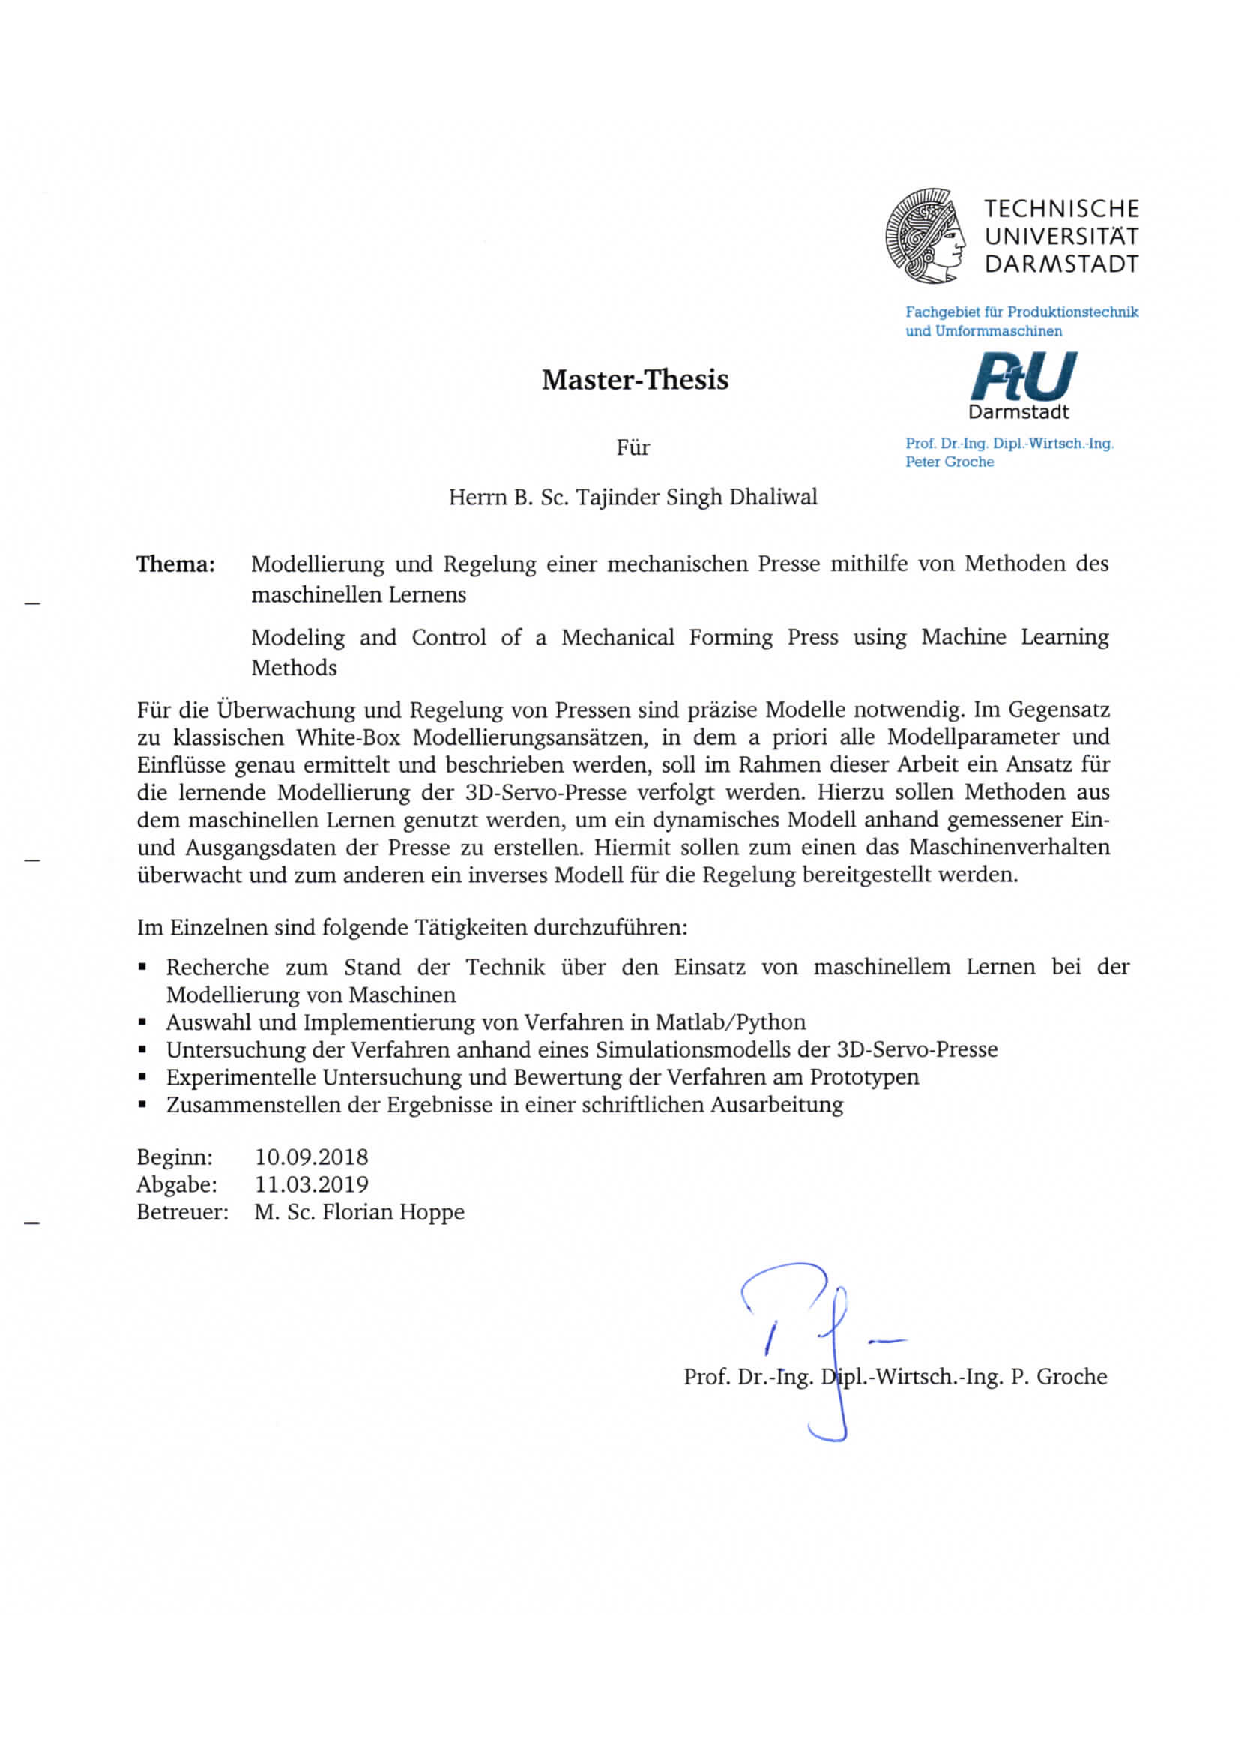
\includepdf[scale=1.0]{common/Aufgabenstellung_cropped}

%\cleardoublepage
%\section*{Aufgabenstellung}
%
Lorem ipsum dolor sit amet, consetetur sadipscing elitr, sed diam nonumy eirmod tempor invidunt ut labore et dolore magna aliquyam erat, sed diam voluptua. At vero eos et accusam et justo duo dolores et ea rebum. Stet clita kasd gubergren, no sea takimata sanctus est Lorem ipsum dolor sit amet. Lorem ipsum dolor sit amet, consetetur sadipscing elitr, sed diam nonumy eirmod tempor invidunt ut labore et dolore magna aliquyam erat, sed diam voluptua. At vero eos et accusam et justo duo dolores et ea rebum. Stet clita kasd gubergren, no sea takimata sanctus est Lorem ipsum dolor sit amet. Lorem ipsum dolor sit amet, consetetur sadipscing elitr, sed diam nonumy eirmod tempor invidunt ut labore et dolore magna aliquyam erat, sed diam voluptua. At vero eos et accusam et justo duo dolores et ea rebum. Stet clita kasd gubergren, no sea takimata sanctus est Lorem ipsum dolor sit amet.   

Duis autem vel eum iriure dolor in hendrerit in vulputate velit esse molestie consequat, vel illum dolore eu feugiat nulla facilisis at vero eros et accumsan et iusto odio dignissim qui blandit praesent luptatum zzril delenit augue duis dolore te feugait nulla facilisi. Lorem ipsum dolor sit amet, consectetuer adipiscing elit, sed diam nonummy nibh euismod tincidunt ut laoreet dolore magna aliquam erat volutpat.   

Ut wisi enim ad minim veniam, quis nostrud exerci tation ullamcorper suscipit lobortis nisl ut aliquip ex ea commodo consequat. Duis autem vel eum iriure dolor in hendrerit in vulputate velit esse molestie consequat, vel illum dolore eu feugiat nulla facilisis at vero eros et accumsan et iusto odio dignissim qui blandit praesent luptatum zzril delenit augue duis dolore te feugait nulla facilisi.   

\vspace{0.5cm}
\begin{tabular}{ll}
Beginn: & \SADABegin \\
Ende:   & \SADAAbgabe \\
Kolloquium:& \SADASeminar
\end{tabular}

\vspace{1cm}

\vfill
%\newpage
{\renewcommand{\baselinestretch}{1} % f�r diesen Abschnitt einfacher Zeilenabstand
\normalsize % anwenden des Zeilenabstandes

%\vspace{5cm}
\begin{minipage}{0.8\textwidth}
	Technische Universitaet Darmstadt\\
	Ptu\\[0.5cm]
%
	Otto-Berndt-Strass 2\\
	64287 Darmstadt\\
	Telefon\\
	
\end{minipage}
\begin{minipage}{0.2\textwidth}
\flushright  % rechtsb�ndig
\ \\[2.7cm]
\SADAlogo\;
\end{minipage}}



\cleardoublepage
\ \\[3cm]	% Diese Zeile erzeugt einen Abstand von 4cm zur ersten Zeile, die nur ein Leerzeichen
			% enth�lt

\section*{Erkl\"arung zur Abschlussarbeit gem\"aß \S\ 22 Abs. 7 und \S\ 23 Abs. 7 APB TU Darmstadt}
\noindent
Hiermit versichere ich, Tajinder Singh Dhaliwal, die vorliegende Master-Thesis gem\"aß \S\ 22 Abs. 7 APB der TU Darmstadt ohne Hilfe Dritter und nur mit den angegebenen Quellen und Hilfsmitteln angefertigt zu haben. Alle Stellen, die Quellen entnommen wurden, sind als solche kenntlich gemacht worden. Diese Arbeit hat in gleicher oder \"ahnlicher  Form noch keiner Pr\"ufungsbeh\"orde  vorgelegen. 

Mir ist bekannt, dass im Falle eines Plagiats (\S\ 38 Abs. 2 APB) ein T\"auschungsversuch vorliegt, der dazu f\"uhrt, dass die Arbeit mit 5,0 bewertet und damit ein Pr\"ufungsversuch verbraucht wird. Abschlussarbeiten d\"urfen nur einmal wiederholt werden.

Bei der abgegebenen Thesis stimmen die schriftliche und die zur Archivierung eingereichte elektronische Fassung gem\"aß \S\ 23 Abs. 7 ABP \"uberein.

Bei einer Thesis des Fachbereichs Architektur entspricht die eingereichte elektronische Fassung dem vorgestellten Modell und den vorgelegten Pl\"anen.
\vspace*{20mm} \\
\noindent
\begin{tabular}{ll}
	Datum: & Unterschrift: \\
	 & \\
	\rule{0.3\textwidth}{0.4pt}	& \rule{0.4\textwidth}{0.4pt}\\
\end{tabular}
	
\vspace{40mm}
\noindent




\clearpage
\section*{Kurzfassung}
Diese Arbeit befasst sich mit der Entwicklung eines Verfahrens zur Beherrschung von Unsicherheiten in Drei-Punkt-Richtprozessen. Beim Richten ist sowohl fue Prozessgeschwindigkeit als auch Prozessgenauigkeit die genaue Praktion der kfederung des Bauteils von entscheidender Rolle. Dabei stellen oftmals schwankende Bauteileigenschaften eine Herausforderung dar,  die eine Regelstrategie benwird, die diese Schwankungen erkennen und kompensieren kann. Hierzu wird in dieser Arbeit ein Verfahren entwickelt, welches es erlicht, parallel zu einem Biegeprozess in Echtzeit alle relevanten Bauteilinformation aus der Kraft-Weg-Messung des Bauteils zu identifizieren und damit zu jedem Zeitpunkt die Rderung zu prktieren.\\
Anhand der Ergebnisse an einer Drei-Punkt-Richtmaschine wird gezeigt, dass mit diesem Verfahren auch ohne Kenntnis der Materialeigenschaften mit nur einem Richthub eine hohe Genauigkeit erzielt werden kann. Daer hinaus werden in Versuchen auch die Grenzen der Robustheit gegener Schwankungen in der Bauteilgeometrie getestet. Als Ausblick zu diesem Verfahren wird ein Lungsansatz geliefert, mit dem ein hes Man vertrauenswiger Information gewonnen werden kann und durch eine stochastische Modellierung der Unsicherheiten eine weitere Optimierunist. 

\textbf{Schter:} Drei-Punkt-Richten, Unsicherheit, Unwissen, Materialeigenschaft, Bauteileigenschaften, Robustheit


\selectlanguage{english}
\section*{Abstract} 

This thesis deals with the development of a method to control uncertainties in three-point straightening processes. Speed and accuracy in straightening processes are determined by its quality of springback prediction. Alternating material and part properties are a challenging task for springback prediction and require a control strategy which is able to detect and compensate those uncertainties. Therefore this thesis presents a method which is able to extract all essential information from the online force-displacement curvature during the straightening process and provides a real-time springback prediction.\\
Results from real processes on a three-point straightening machine have shown that this method is able to handle unknown uncertainties in material properties and achieve a high accuracy within one stroke. Additional results show the robustness of this method and its limits regarding uncertainties in part properties. A further solution is provided which gives an outlook on how to increase the amount of available, reliable information and therefore optimize the method with a stochastic uncertainty.

\textbf{Keywords:} three-point straightening, stochastic uncertainty, unknown uncertainty, material properties, part properties, robustness
\selectlanguage{ngerman} 
% =================================================================================

% =================================================================================
% Inhaltsverzeichnis
% =================================================================================
\cleardoublepage	% Auf einer leeren rechten Seite beginnen
\phantomsection		% Diese und die nächste Zeile dient dazu, für das Inhalts-
					% verzeichnis einen Eintrag in das pdf-Inhaltsverzeichnis,
					% aber nicht in das normale Verzeichnis zu erzeugen.
\pdfbookmark[0]{\contentsname}{pdf:toc}	
\setcounter{secnumdepth}{3}
\setcounter{tocdepth}{3} 
\tableofcontents	% Inhaltsverzeichnis einfügen
\clearpage	% Sonst kommt nichts mehr auf die Seite
% =================================================================================


% =================================================================================
% Symbole und Abkürzungen
% =================================================================================
% Nach dem Inhaltsverzeichnis kommt ein Verzeichnis der häufig verwendeten
% Symbole und Abkürzungen. Dazu kann man das Paket 'nomencl' verwenden, oder man
% erstellt es von Hand.
\chapter*{Symbole und Abkzungen}
\addcontentsline{toc}{chapter}{Symbole und Abkungen} % erzeugt einen Eintrag im Inhaltsverzeichnis
%
\paragraph*{Operatoren und Funktionen}
\begin{tabularx}{\textwidth}{@{}l@{\qquad}X@{\quad}p{18mm}}
\toprule
	Symbol & Beschreibung & \\ \midrule
	$*$ & Faltung\\
	$\star$ & Kreuzkorrelation\\
	$\delta(\cdot)$ & Dirac-Funktion\\
	$\frac{\partial f}{\partial x}$ & partielles Differential\\
	$\frac{\mrm{d} f}{\mrm{d} t}$ & totales Differential\\
	$\Theta(\cdot)$ & Heaviside-/Sprung-Funktion\\
\end{tabularx}
%
\paragraph*{Lateinische Symbole und Formelzeichen}
\begin{longtable}{@{}l@{\qquad}p{0.72\columnwidth}@{\quad}p{18mm}}
\toprule
%K�rzel 	& vollst�ndige Bezeichnung 							\\ \midrule
Symbol & Beschreibung & Einheit\\ \midrule
\endfirsthead
\toprule
%K�rzel 	& vollst�ndige Bezeichnung 							\\ \midrule
Symbol & Beschreibung & Einheit\\ \midrule
\endhead

%\begin{tabularx}{\textwidth}{@{}l@{\qquad}X@{\quad}p{18mm}}
%\toprule
	%Symbol & Beschreibung & Einheit\\ \midrule
	$A$ & Bauteilfl in der $x$-$z$-Ebene & $\mrm{mm}^2$ \\
	$a_\mrm{f}$ & Parameter der Kaltflieurve & $\ufrac{N}{mm^2}$\\
	$b$ & Integrationskonstante & N\\
	$b_\mrm{f}$ & Parameter der Kaltflieve & $\ufrac{N}{mm^2}$\\
	$E$ & Elastizitsmodul & $\ufrac{N}{mm^2}$\\
	$F$ & aktuelle Reaktionskraft des Bauteils & N\\
	$F_m$ & Reaktionskraft des Bauteils zu Beginn der $m$-ten Entlastung & N\\
	$\bar{F}_m$ & Reaktionskraft des Bauteils nach der $m$-ten Entlastung & N\\
	$F_n$ & Reaktionskraft des Bauteils im $n$-ten Abtastschritt & N\\
	$\ve{F}_{1:n}$ & Vektor der Reaktionskre vom ersten bis $n$-ten Abtastschritt & N\\
	$\FY$ & Bauteilflieenze & N\\
	$h$ & Bauteilhe & mm\\
	$\Iy$ & Flentrsmoment um die $y$-Achse & $\mrm{mm}^4$\\
	$k$ & Bauteilsteifigkeit & $\ufrac{N}{mm}$\\
	$\khat$ & gescte Bauteilsteifigkeit & $\ufrac{N}{mm}$\\
	$\khatel$ & verbesserte Scung der Bauteilsteifigkeit & $\ufrac{N}{mm}$\\
	$\khatpl$ & geschtes Tangentenmodul im plastischen Bereich & $\ufrac{N}{mm}$\\
	$\khatelm$ & verbesserte Schng der Bauteilsteifigkeit nach der $m$-ten Rderung & $\ufrac{N}{mm}$\\
	$k_\mrm{f}$ & Fliepannung der Kaltfliee & $\ufrac{N}{mm^2}$\\
	$l$ & Bauteille & mm\\
	$l_\mrm{eff}$ & effektive Bauteillge zwischen den Auflagern & mm\\
	$M_\mrm{y}$ & Biegemoment um die $y$-Achse & Nmm\\
	$t$ & Zeit & s\\
	$\Tabt$ & Abtastzeit der Ein- und Ausge & s\\
	$U$ & Steuerspannung des Proportionalventils & V\\
	$\dot{V}$ & Volumenstrom durch das Proportionalventil & $\ufrac{mm^3}{s}$\\
	$w$ & aktuelle Bauteildurchbiegung & mm\\
	$w_n$ & Bauteildurchbiegung im $n$-ten Abtastschritt & mm\\
	$w_m$ & Bauteildurchbiegung zu Beginn der $m$-ten Entlastung & mm\\
	$\ve{w}_{1:n}$ & Vektor der Bauteildurchbiegungen vom ersten bis $n$-ten Abtastschritt & mm\\
	$\dot{w}$ & aktuelle Biegegeschwindigkeit & $\ufrac{mm}{s}$\\
	$\wOhat$ & geschte Bauteildurchbiegung nach Entlastung & mm\\
	$\wO$ & Bauteildurchbiegung nach Entlastung & mm\\
	$\wO_m$ & Bauteildurchbiegung nach der $m$-ten Entlastung & mm\\
	$\wOsoll$ & Solldurchbiegung des Bauteils nach Entlastung & mm\\
	$w_0$ & Anfangsbauteildurchbiegung & mm\\
%\end{tabularx}
\end{longtable}
%%
\paragraph*{Griechische Symbole und Formelzeichen}
%\begin{longtable}{ll@{\qquad}X@{\quad}p{18mm}}
\begin{longtable}{@{}l@{\qquad}p{0.72\columnwidth}@{\quad}p{18mm}}
\toprule
Symbol & Beschreibung & Einheit\\ \midrule
\endfirsthead
\toprule
Symbol & Beschreibung & Einheit\\ \midrule
\endhead
%\begin{tabularx}{\textwidth}{@{}l@{\qquad}X@{\quad}p{18mm}}
%\toprule
	%Symbol & Beschreibung & Einheit\\ \midrule
	$\epsilon$ & Rauschprozesses der Kraftmessung & N\\
	$\varepsilon$ & mechanische Dehnung & \\
	$\varepsilon_\mrm{el}$ & elastische Dehnung & \\
	$\varepsilon_\mrm{pl}$ & plastische Dehnung & \\
	$\eta$ & Verfestigungsexponent des Bauteils\\ 
	$\eta_\mrm{f}$ & Verfestigungsexponent der Kaltflieve &\\ 
	$\lambda$ & Vergessensfaktor & \\
	$\mu_\mrm{R}$ & Reibungskoeffizient & \\
	$\Bmu$ & Mittelwertvektor der Zufallsvariablen $k$ und $b$ & \\
	$\nu$ & Rauschprozess der Wegmessung & \\
	$\rho_0$ & Krgsradius des Balkens & \\
	$\BSigma$ & Kovarianzmatrix der Zufallsvariablen $k$ und $b$ & \\
	$\sigma$ & mechanische Spannung & $\ufrac{N}{mm}$\\
	$\sigma^2_\epsilon$ & Varianz der Kraftmessung & $\mrm{N}^2$\\
	$\sigma^2_\nu$ & Varianz der Wegmessung & $\mrm{mm}^2$\\
	$\sigma^2_\mrm{F}$ & Varianz der Zufallsvariable $F$ & $\mrm{N}^2$\\
	$\sY$ & Materialflierenze & $\ufrac{N}{mm}$\\
	$\varphi$ & Umformgrad & \\
%\end{tabularx}
\end{longtable}

\newpage
\paragraph*{Abkungen}

\LTXtable{\textwidth}{inc/Abkuerzungen}

\cleardoublepage

%% =================================================================================
%% Abbildungsverzeichnis
%% =================================================================================
\cleardoublepage
\phantomsection					% Für Aufnahme ins Inhaltsverzeichnis
\addcontentsline{toc}{chapter}{\listfigurename}	% In Inhaltsverzeichnis von
												% Dokument und pdf aufnehmen
\listoffigures
%% =================================================================================
%
%% =================================================================================
%% Tabellenverzeichnis
%% =================================================================================
\cleardoublepage
\phantomsection					% Für Aufnahme ins Inhaltsverzeichnis
\addcontentsline{toc}{chapter}{\listtablename}	% In Inhaltsverzeichnis von
												% Dokument und pdf aufnehmen
\listoftables
%% =================================================================================

% =================================================================================
% Hauptteil
% =================================================================================
\cleardoublepage
\phantomsection					% Für Aufnahme ins Inhaltsverzeichnis
\pagenumbering{arabic}	% Hauptteil bekommt arabische Seitenzahlen


\chapter{Einführung}

Die Planung und Einführung von Fertigungssystemen geht mit Unsicherheiten einher. Dies ist bedingt durch die limitierte Gültigkeit von Annahmen in Bezug auf zukünftige Ereignisse während der Auswahl- und Entwicklungsphase von Fertigungstechnologien und Werkzeugmaschinen \cite{Groche.2010}. Nach \cite{Gerwin.1993} gibt es vier Arten von Unsicherheiten: die Marktakzeptanz von bestimmten Produkten, die Länge der Produktlebensphasen, spezifische Produkteigenschaften und die aggregierte Produktnachfrage. Ein mögliches Lösungskonzept zur Bewältigung dieser Unsicherheiten besteht darin, die Flexibilität von Fertigungssystemen zu erhöhen. Daraus ergeben sich nach \cite{Son.1987} folgende Vorteile: durch die Erhöhung dieser können erstens eine höhere Anzahl an Produkten und Produktvariationen (Werkzeugflexibilität) in den Fertigungsprozess integriert werden, zweitens erhöht sich die Adaptionsfähigkeit des Fertigungsprozesses auf eine Veränderung der Produktpalette (Produktflexibilität), drittens erhöht sich bei flexiblen Fertigungsprozessen die Adaptionsfähigkeit auf Veränderungen des Prozesses, z.B. durch technologische Entwicklungen (Prozessflexibilität) und viertens kann durch solche Fertigungssysteme flexibler auf Nachfrageschwankungen reagiert werden (Nachfrageflexibilität). \\ 

Bisher kommen Umformmaschinen vor allem bei großen Stückzahlen und ausgewählten Umformmethoden oder kleinen Stückzahlen und vorher speziell festgelegten Werkzeugverfahrwegen zum Einsatz \cite{Groche.2010}. Dadurch ist die Adaptionsfähigkeit auf Nachfrageschwankungen sehr eingeschränkt \cite{Schmoeckel.1991}. Dagegen bietet bringt die Integration von Servomotoren in Pressen neue Möglichkeiten der Flexibilisierung mit \cite{Groche.2004}. Um dem Anspruch einer höheren Flexibilität für Pressen gerecht zu werden, entwickelte das Institut für Produktionstechnik und Umformmaschinen (PtU) die   neuartige 3D-Servo-Presse. Diese verfügt über drei Antriebssysteme. Diese erlauben es der 3D-Servo-Presse, zuzüglich zur translatorischen Stößelbewegung eine Verkippung orthogonal zur Translationsbewegung durchzuführen. Dadurch ergeben sich insgesamt drei Freiheitsgrade: eine translatorische Hubbewegung und zwei rotatorische Kippbewegungen. Dadurch ist die Herstellung neuartiger Produktgeometrien und das Einbringen bestimmter Materialeigenschaften in den umgeformten Produkten durch definierte Werkzeugbewegungen denkbar. Beispielsweise lässt sich durch den Einsatz der 3D-Servo-Presse die Anzahl der Prozessschritte bei der Herstellung von Bauteilen mit sehr hohen Umformgraden durch die gezielte Steuerung des Materialflusses reduzieren \cite{Sinz.2018}. Durch den Einsatz der 3D-Servo-Presse soll damit dem Anspruch nach höherer Flexibilisierung und der damit einhergehenden höheren Wirtschaftlichkeit gerecht werden. \\

Zusätzlich zum Thema Flexibilisierung von Fertigungssystemen hat sich das Thema Industrie 4.0 als weiterer Forschungsgegenstand in der Literatur etabliert. Nach \cite{VDMA.2018} stellt die Integration von Sensoren und die damit ermöglichte Zustandsüberwachung einer Werkzeugmaschine ein Teilaspekt der Industrie 4.0 dar. Durch die Zustandsüberwachung ist eine frühzeitige Detektion von Ausfällen möglich. Darüber hinaus können durch die Erfassung des Betriebszustandes Prognosen zur zukünftigen Funktionsfähigkeit der Werkzeugmaschine gemacht werden. Diese erlauben im weiteren Verlauf das Initiieren von Maßnahmen zur Behebung von möglich auftretenden Ausfällen, Defekten etc. \cite{VDMA.2018} \\

Sowohl für die Regelung der 3D-Servo-Presse während des normalen Betriebsfalles als auch für die Zustandsüberwachung der 3D-Servo-Presse ist eine Modellbildung dieser notwendig. Im Gegensatz zu vergangenen Arbeiten kommt in diesiger Arbeit kein White-Box-Ansatz, in dem a priori alle Modellierungsparameter und Einflüsse genau ermittelt werden, sondern ein Blackbox-Ansatz zur Anwendung. Für die Parametrisierung des Black-Box-Modells kommen Methoden des maschinellen Lernens zum Einsatz, um anhand gemessener Eingangs- und Ausgangsgrößen ein dynamisches Modell zu erstellen. Auf Basis dieses Modells sollen Konzepte zur Zustandsüberwachung als auch zur Regelung der 3D-Servo-Presse entwickelt werden. Als Grundlage dieser Arbeit dient der Prototyp der 3D-Servo-Presse. Diese steht als Forschungsobjekt am PtU an der Technischen Universität Darmstadt zur Verfügung. \\

\section{Abgrenzung zu vorherigen Arbeiten}
\label{cha:Abgrenzung}
Wie bereits erwähnt verfügt die 3D-Servo-Presse über drei Servo-Motoren, welche die Antriebsmomente liefern. Mit der Hilfe von ungleich übersetzenden Koppelgetrieben werden nicht nur die Drehmomente in die auf den Stößel wirkende Zustellkraft übersetzt, sondern auch eine Kippbewegung des Stößels in zwei rotatorische Freiheitsgraden ermöglicht. Für diese Presse sind in mehreren Vorarbeiten bereits Pressenmodelle entwickelt worden. \\

\cite{Rakowitsch.2018} entwickelte in seiner Arbeit ein mechanisches Mehrkörpermodell des Getriebes der 3D-Servo-Presse. Bei diesem Pressenmodell berücksichtigt er sowohl die Nachgiebigkeiten als auch die Massenträgheiten aller Getriebeglieder, um damit dynamische Vorgänge, wie z.B. Schwingungen und das Verfahren der Getriebestellung, zu untersuchen. \cite{Rakowitsch.2018} kommt zum Ergebnis, dass das Mehrkörpermodell steifer ist als das reale Getriebe. Nach einer erneuten Parameteridentifikation zeigte sich in den Messdaten eine Hysterese und mechanisches Spiel. Nach \cite{Rakowitsch.2018} konnten diese nicht durch das Modell abgebildet werden. Weiterhin kommt \cite{Rakowitsch.2018} zum Schluss, dass die aus der Identifikation entspringenden Parameter einer Unsicherheit unterliegen. Daraufhin untersuchte \cite{Rakowitsch.2018} die Auswirkungen der Parameterunsicherheit und wählte aus den unsicheren Parametern zwei Parametersätze, aus welchen zwei Grenzmodelle hervorgingen, ein weiches und steifes Pressenmodell. Mit diesen konnte \cite{Rakowitsch.2018} letztlich die Zustandsüberwachung durchführen. \\

In dieser Arbeit soll nun im Gegensatz zu \cite{Rakowitsch.2018} ein Black-Box-Modell an Stelle eines White-Box-Modells entwickelt werden. Die Parametrisierung des Modells findet dabei über Methoden des maschinellen Lernens statt. Das Ziel besteht darin, bisher in White-Box-Modellen nicht abgebildete Effekte, wie z.b. die nicht lineare Reibung, Fertigungstoleranzen, statische Dehnungen, Lagerreibung, Abnutzungserscheinungen, etc. durch Methoden des maschinellen Lernens abzubilden.


\section{Vorgehensweise}








   





\chapter{Stand der Technik}

Das Ziel dieser Arbeit besteht darin, ein Ersatzmodell für den Prototypen der 3D-Servo-Presse zu entwickeln. Die Parametrisierung erfolgt über Methoden des maschinellen Lernens. Auf Basis des Ersatzmodells folgt im weiteren Verlauf die Entwicklung von Konzepten zur Zustandsüberwachung und Regelung der 3D-Servo-Presse. Zunächst soll jedoch auf die Grundlagen der Modellbildung eingegangen werden.

\section{Modellierungsansätze}
\label{cha:modell}

Nach \cite{Isermann.2011} gibt es mehrere Möglichkeiten der Modellbildung, die theoretische, die experimentelle und theoretisch-experimentelle Mischformen. Zunächst erfolgt die Beschreibung der theoretischen Modellbildung. \\ 
Bei der theoretischen Modellierung findet die Beschreibung des Systems entweder über partielle oder gewöhnliche Differentialgleichungen statt. Da reale Systeme in vielen Fällen zu komplex und/oder kompliziert sind, ist es üblich, das Modell zu vereinfachen, z.B. durch das Ignorieren bestimmter real auftretender Effekte (z.B. nichtlineare Reibungseffekte). In der Regel ist es nach \cite{Isermann.2011} möglich, das Modell durch vier Arten von Gleichungen zu beschreiben:

\begin{itemize}
	
	\item \textit{Bilanzgleichungen:} Dazu gehören die Massen-, Energie- und Impulserhaltung.
	\item \textit{Physikalische oder chemische Zustandsgleichungen:} Diese sogenannten konstitutiven Gleichungen beschreiben reversible Vorgänge, wie z.B. das 2. Newtonsche Gesetz.
	\item  \textit{Phänomenologische Gleichungen:} Diese  beschreiben irreversible Vorgänge, wie z.B. Reibung.
	\item  \textit{Verbindungsgleichungen:} Dazu gehören die Kirchhoffschen Regeln, Momentengleichgewichte, etc. \cite{Isermann.2011}
	
\end{itemize} 

Nach \cite{Isermann.2011} setzt sich die theoretische Modellbeschreibung des Systems aus einer Mehrzahl von Gleichungen zusammen. Die Lösung des Gleichungssystems ist zwar explizit nicht immer möglich, aber trotzdem können individuelle Gleichungen wichtige Anhaltspunkte bezüglich der Modellstruktur liefern. \cite{Isermann.2011} \\
Die experimentelle Modellbildung basiert auf Messdaten, welche im Zuge von Versuchen aufgenommen werden. Die Messdaten teilen sich auf in Eingangs- und Ausgangsgrößen des Systems. Als Eingangsgrößen können entweder reale Eingangsstellgrößen oder künstlich erzeugte Testsignale mit bestimmten Eigenschaften fungieren. Im Fall der 3D-Servo-Presse seien der Exzentervorschub und die beiden Spindelvorschübe die Eingangsgrößen des Systems, da sie die Höhenverstellung des Stößels als Ausgangsgröße festlegen. Das Ziel der theoretischen Modellbildung besteht nun darin, für eine ausgewählte Modellstruktur die Parameter so zu identifizieren, dass ein möglichst guter Zusammenhang zwischen Eingangs- und Ausgangsgrößen hergestellt wird. Der dafür in der Literatur standardmäßig verwendete Begriff ist Systemidentifikation. \cite{Isermann.2011} \\
Die Bezeichnung der Modellstruktur, welche aus der theoretischen Modellbildung hervorgeht, lautet White-Box-Modell. Das Gegenstück dazu ist das Black-Box-Modell, welches aus der experimentellen Modellbildung hervorgeht. Nach \cite{Isermann.2011} haben White-Box- und Black-Box-Ansätze verschiedene Vor- und Nachteile, aber dennoch sind die komplementär zueinander. Um Vorteile beider Modellierungsansätze zu vereinen, sind ebenfalls sogenannte Gray-Box-Modell-Ansätze in verschiedenen Abstufungen (Light-Gray-Box-Modell, Dark-Gray-Box-Modell) entstanden. Eine Übersicht über alle Modellierungsansätze liefert Abbildung \ref{fig:modeling_methods}. Die wesentlichen Eigenschaften beider Modellierungsansätze sind in Tabelle \ref{tab:modeling_methods} zu finden. 




\begin{longtable}{p{7.0cm} p{7.0cm}}
	\caption{Eigenschaften theoretischer und experimenteller Modellierungsansätze \cite{Isermann.2011}} \\ \toprule
	% Definition des Tabellenkopfes auf der ersten Seite
	\textbf{Theoretische Modellbildung} & \textbf{Experimentelle Modellbildung (Systemidentifikation)} \\
	\hline
	\endfirsthead % Erster Kopf zu Ende
	% Definition des Tabellenkopfes auf den folgenden Seiten
	\caption{Lange Tabelle mit Longtable Fortsetzung}\\
	1 Spalte & 2 Spalte\\
	\hline
	\endhead % Zweiter Kopf ist zu Ende
	\hline
	
	% Ab hier kommt der Inhalt der Tabelle
	Modellstruktur folgt Naturgesetzen & Modellstruktur muss angenommen werden\\ \hline
	Modellierung des Übertragungsverhaltens und innerer Systemvorgänge & lediglich Identifizierung des Übertragungsverhaltens\\ \hline
	Gültigkeit des Modells für eine Reihe von Prozessen ähnlichen Types und unterschiedlicher Randbedingungen & Modell ist nur für das untersuchte System innerhalb der Betriebsgrenzen gültig\\ \hline
	Modellkoeffizienten sind nicht exakt bekannt & exaktere Bestimmung der Modellkoeffizienten für das gegebene System innerhalb der Betriebsgrenzen\\ \hline
	Modell kann für nicht existente Systeme entwickelt werden & Modell kann nur für ein bereits existierendes System entwickelt werden\\ \hline
	das interne Systemverhalten muss bekannt und mathematisch beschreibbar sein & Identifikationsmethoden sind unabhängig vom untersuchten System und können auf andere Systeme angewendet werden\\ \hline
	üblich langsamer Prozess mit hohem Zeitaufwand & schneller Prozess bei bereits bekannten Identifikationsmethoden\\ \hline
	Modelle können sehr komplex und detailliert ausfallen & Modellgröße kann auf den Anwendungsfall des Modells angepasst werden\\
	\bottomrule
	\label{tab:modeling_methods} 
\end{longtable}


\begin{figure} 
	\centering
	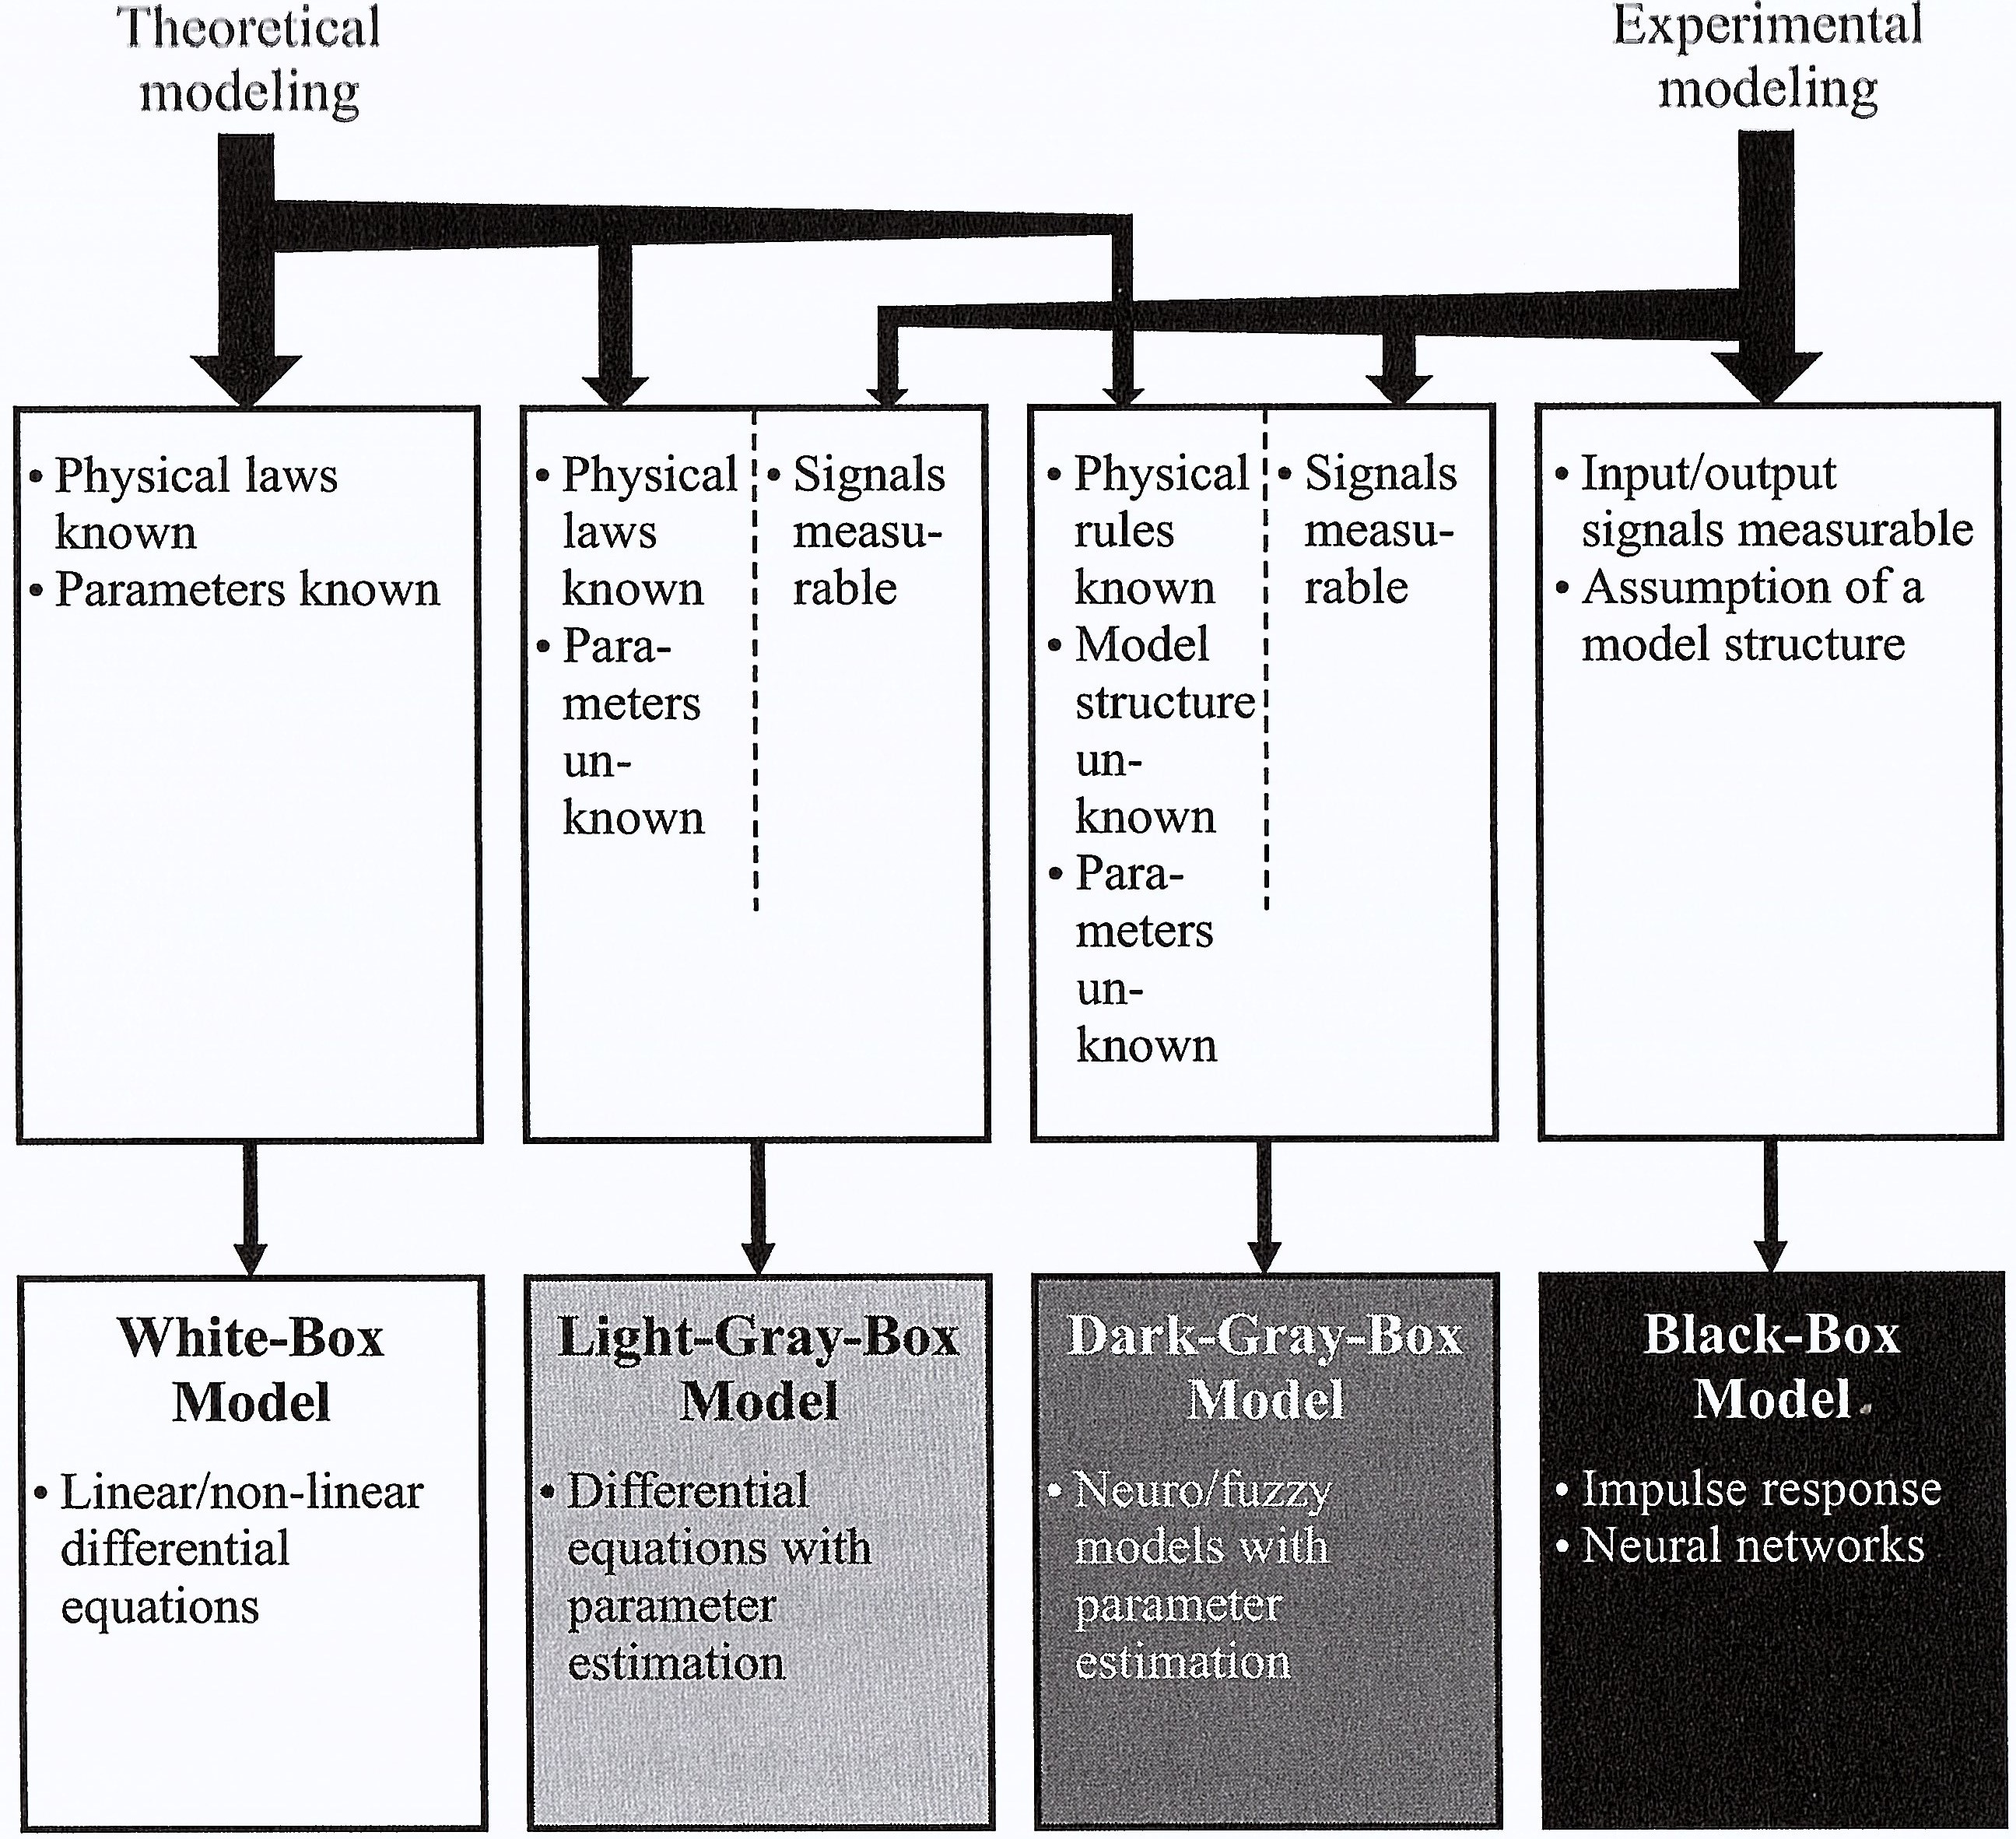
\includegraphics[width=0.75\textwidth]{images/modeling_methods}
	\caption{Mathematische Modelle von White-Box- bis zu Black-Box-Modellen \cite{Isermann.2011}}
	\label{fig:modeling_methods}
\end{figure}

Wie in Tabelle \ref{tab:modeling_methods} zu erkennen ist, umgehen Black-Box-Modelle einen wesentlichen Nachteil von White-Box-Modellen, nämlich die exakte Kenntnis der internen Systemzusammenhänge, das Aufstellen von mathematischen Gleichungen zur Beschreibung dieser und die explizite Lösung des Gleichungssystems. Für komplexe Systeme  wie der 3D-Servo-Presse stößt der White-Box-Ansatz auf viele Probleme, siehe Abschnitt \ref{cha:Abgrenzung}. 
Deshalb fungiert das Black-Box-Modell als Grundlage für die Modellbildung des Prototypen der 3D-Servo-Presse.  Wie in Abbildung \ref{fig:modeling_methods} zu erkennen ist, können  Neuronale Netze als Methode zur Parameteridentifikation von Black-Box-Modellen dienen. Neuronale Netze stellen ein Teilgebiet des Maschinellen Lernens dar. Die Grundlagen der Neuronalen Netze werden in Kapitel QUELLE beschrieben. Das Black-Box-Modell dient als Grundlage für die Regelung und die Zustandsüberwachung der 3D-Servo-Presse. Zunächst sollen im nächsten Abschnitt die Grundlagen der Regelung vermittelt werden. 












\section{Regelung}


Die in Abschnitt \ref{cha:modell} vorgestellten Modellierungsansätze haben den Zweck, ein reales System, wie z.B. die 3D-Servo-Presse, in ein Ersatzmodell zu überführen. Dieses hat den Zweck, einen möglichst guten mathematischen Zusammenhang zwischen den Eingangs- und Ausgangsgrößen des realen Systems zu liefern. \\
Nach \cite{Lunze.2013} wirken Eingangsgrößen (z.B. Spindel- und Exzentervorschübe) auf das System ein und verursachen zeitliche Veränderungen des Systems. Die Ausgangsgrößen (z.B. die Position des Stößels) dagegen beschreiben das Systemverhalten als Reaktion auf die Eingangsgrößen. Da sich dabei Kenngrößen des Systems zeitlich verändern, ergibt sich für solchen der Begriff \textit{Dynamisches System}. Nach \cite{Lunze.2013} besteht die Aufgabe der Regelungstechnik nun darin, für ein solches dynamisches System die beeinflussbare Größe $u(t)$ (Stellgröße bzw. Eingangsgröße) so anzupassen, dass ein Regelungsziel $w(t)$ (Führungsgröße bzw. Sollwert) erreicht wird, siehe Abbildung \ref{fig:regelkreis}.

\begin{figure} 
	\centering
	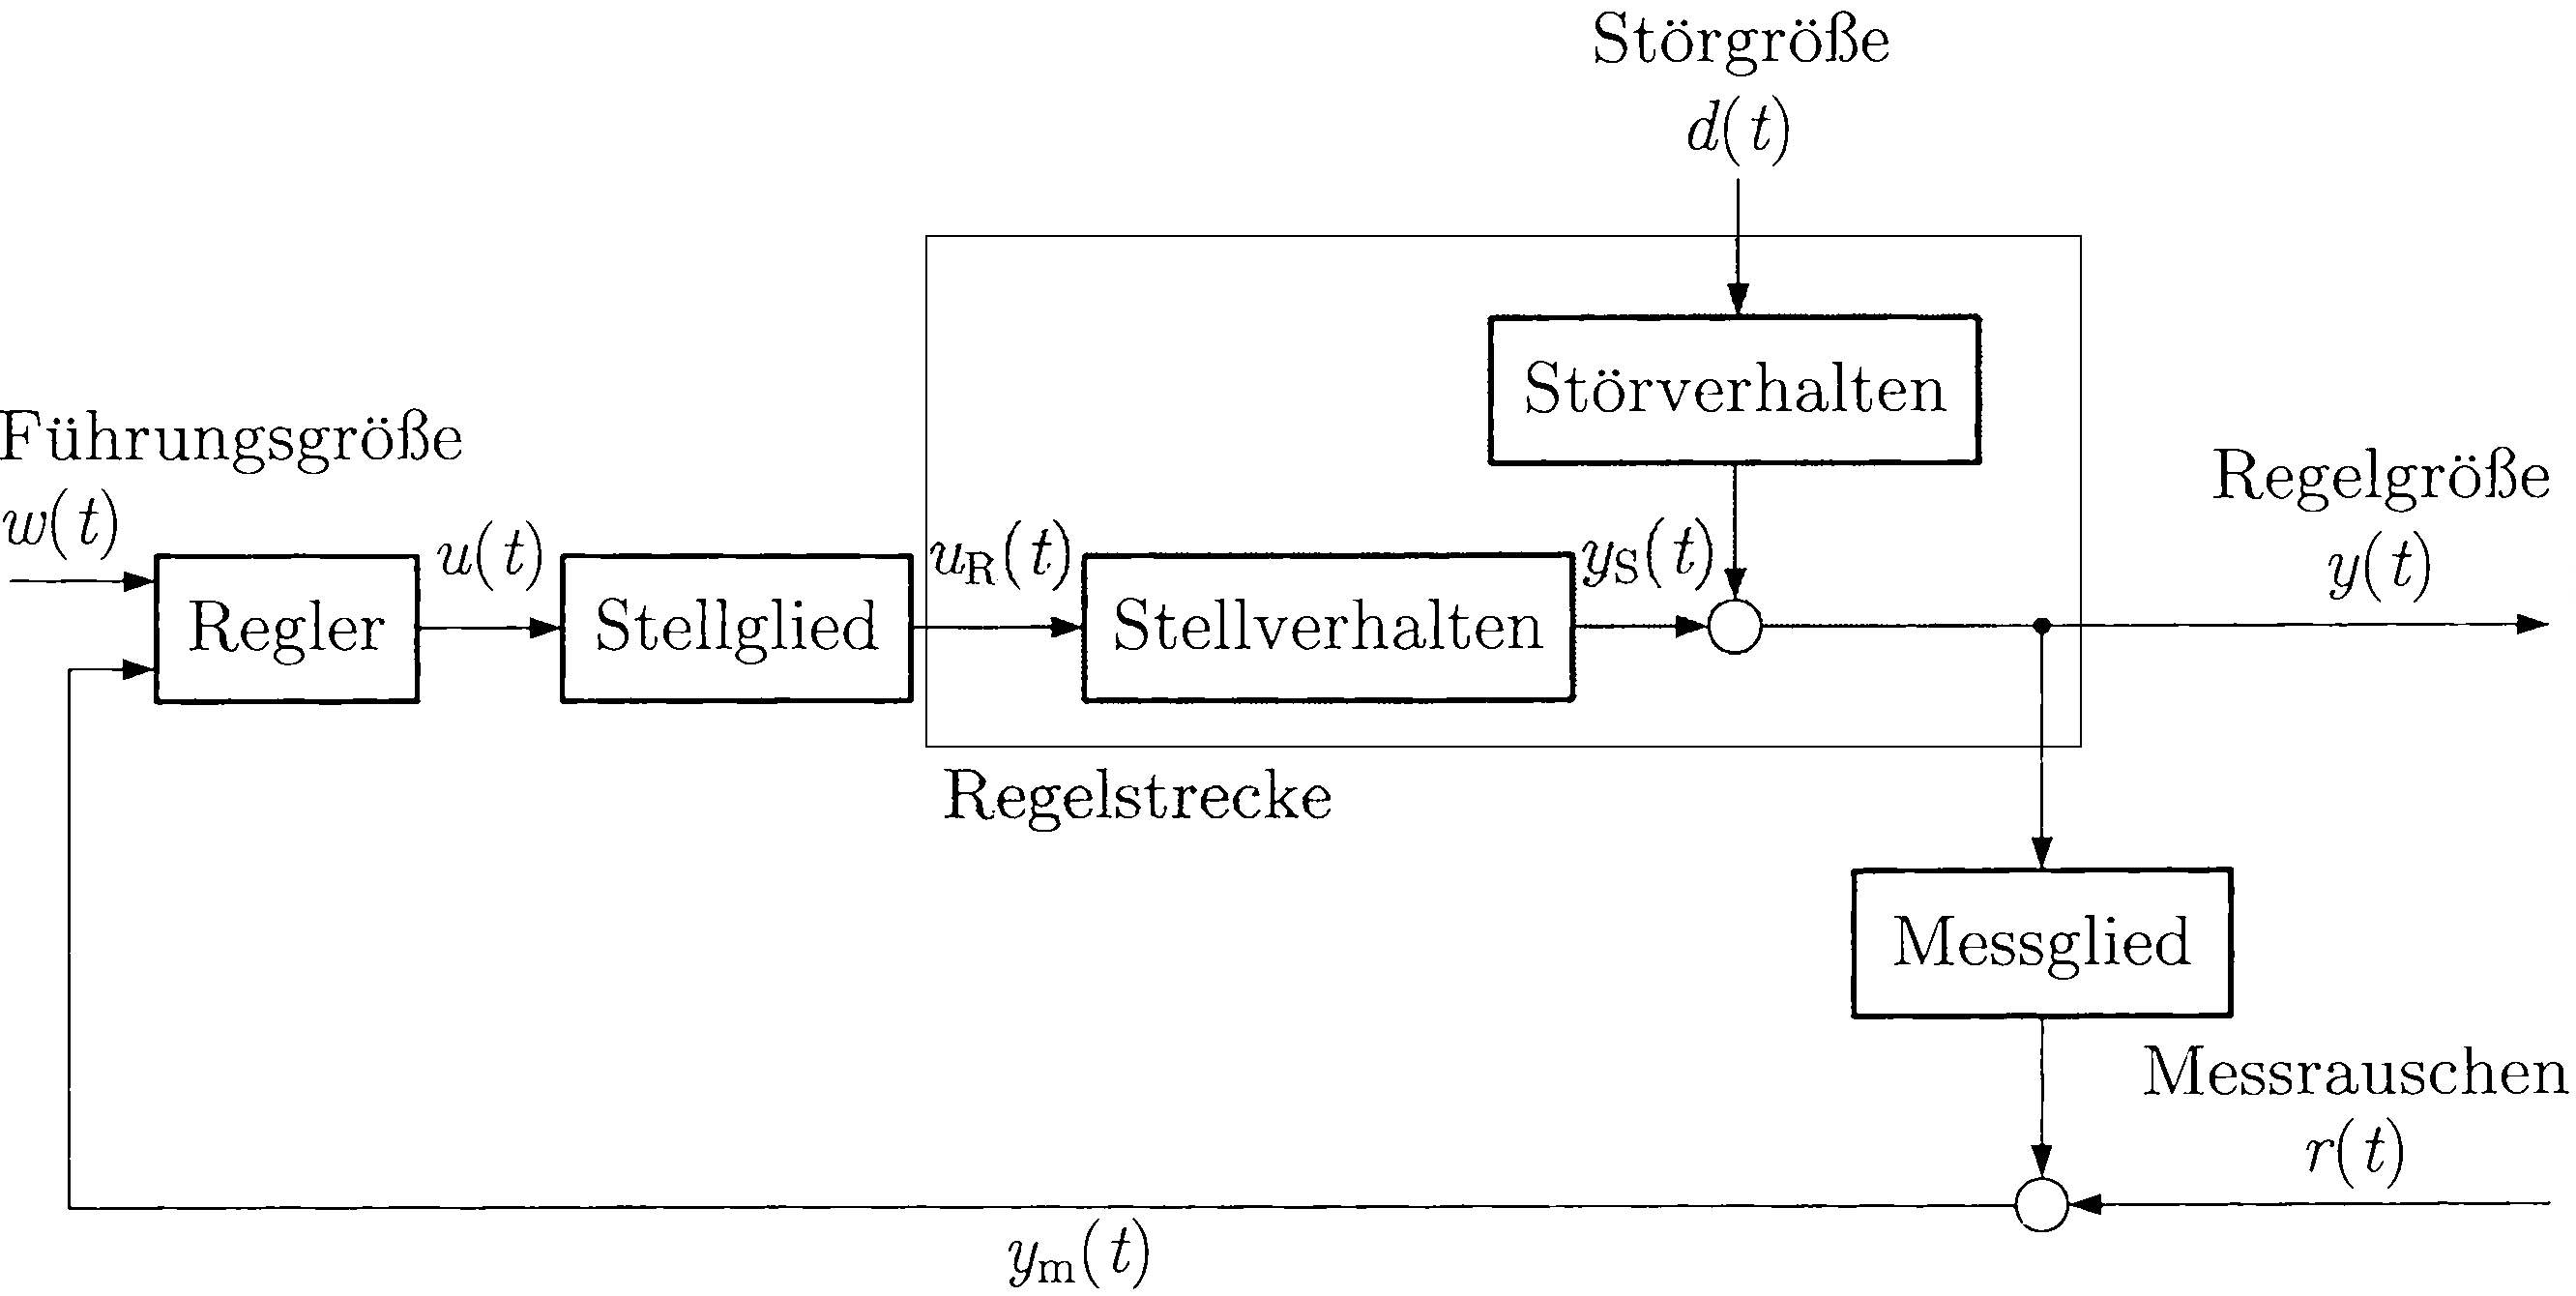
\includegraphics[width=0.75\textwidth]{images/Regelkreis}
	\caption{Erweiterte Grundstruktur des Regelkreises \cite{Lunze.2013}}
	\label{fig:regelkreis}
\end{figure}




Dabei erfüllt die Regeleinrichtung die Aufgabe, unter Nutzung der gemessenen Werte für die Regelgröße (Ausgangsgröße) $y(t)$ die Stellgröße (Eingangsgröße) $u(t)$ so vorzugeben, dass die Differenz zwischen der gemessen Regelgröße (Ausgangsgröße) $y(t)$ und Führungsgröße $w(t)$ minimal ist.  Die Bezeichnung dieser Differenz lautet Regelabweichung $e(t)$, anhand derer die Regeleinrichtung die Stellgröße $u(t)$ zweckmäßig vorgibt. \cite{Lunze.2013}
  
\begin{equation}
e(t) = w(t) - y(t)
\end{equation}


Laut \cite{Lunze.2013} gibt es häufig eine Differenz zwischen der Regelgröße $y(t)$ und der gemessenen Regelgröße $y_m(t)$, da das Messglied selbst über dynamische nichtlineare Eigenschaften verfügt. Dasselbe gilt für Stellglieder (z.B. ein Servomotor, welcher eine Spindel antreibt), welche darüber hinaus sich häufig durch dynamisches Verhalten auszeichnen. Als Resultat ergibt sich daraus eine Differenz zwischen der vorgegeben Stellgröße $u(t)$ und der für den Prozess wirksamen Stellgröße $u_R(t)$. Diese verursacht eine zeitliche Veränderung des Systems (z.B. Stößelbewegung) und erzeugt somit ein Stellverhalten, welches sich mit einem Störverhalten, hervorgerufen durch die unbekannte Störgröße $d(t)$, überlagert. \cite{Lunze.2013} \\ 
Die Auslegung der Regelstrecke muss nun derartig gestaltet sein, dass sie trotz des dynamischen Verhaltens von Messgliedern und Stellgliedern eine minimal mögliche Differenz zwischen der Regelgröße $y(t)$ und Führungsgröße $w(t)$ einstellt. Dafür ist die Auslegung des Reglers entscheidend. \\ 
Für die Auslegung des Reglers ist der Einsatz von Ersatzmodellen notwendig, welche das Systemverhalten des realen Systems so gut wie möglich abbilden. Wie bereits in Abschnitt \ref{cha:Abgrenzung} diskutiert, ist der Einsatz von White-Box-Modellen als Ersatzmodell mit Problemen verbunden. Diese versuchen durch Modellvereinfachungen das Systemverhalten mathematisch zu beschreiben. Damit können sie aber maximal das Stellverhalten des Systems, aber nicht das durch die unbekannte Störgröße $d(t)$ hervorgerufene Störverhalten abbilden. Black-Box-Modelle dagegen, welche mit den Methoden des maschinellen Lernens parametrisiert sind, können auch das Störverhalten mit abbilden, da die Parametrisierung über gemessene Daten stattfindet. Ein Black-Box-Modell, welches das reale Systemverhalten genau genug beschreibt, kann neben der Auslegung von Reglern oder als Hilfsglied im Regelkreis auch im Bereich der Zustandsüberwachung zum Einsatz kommen. Die Grundlagen der Zustandsüberwachung sind im nächsten Abschnitt erläutert.





\input{inc/Stand_der_Technik_Zustandsüberwachung.tex}
\section{Maschinelles Lernen}
\label{cha:machine_learning}

Wie bereits erwähnt, soll die Parametrisierung des in dieser Arbeit entwickelten Black-Box-Modells mit Methoden des maschinellen Lernens stattfinden. Da der Begriff des maschinellen Lernens ein weites Spektrum an theoretischen Grundlagen und praktischen Anwendungen umfasst, enthält der nächste Abschnitt grundlegende Erläuterungen zu diesem Begriff.

Der Begriff des maschinellen Lernens ist ein Oberbegriff, welcher eine Reihe von Methoden umfasst, welche den Zweck haben, Modelle auf Basis von gesammelten bzw. gemessenen Daten zu generieren. Je umfangreicher dabei die Datengrundlage ist, desto besser ist das Modell in der Lage, das Verhalten des realen Systems abzubilden.  Darüber hinaus ist das erzeugte Modell fähig, das Systemverhalten über die verwendete Datengrundlage hinweg zu verallgemeinern. Damit ist die Anwendung des Modells auf bisher unbekannte Datensätze derselben Art möglich, um daraus z.B. Vorhersagen über das zukünftige Systemverhalten zu machen.  Der entscheidende Unterschied zu klassischen Systemidentifikationsmethoden ist, dass die Parametrisierung des Modells automatisiert durch Algorithmen und nicht durch explizites Festlegen stattfindet. \cite{Duriez.2017} \\

Gemeinhin wird in der Literatur die Parametrisierung bzw. Adaptierung der Modelle durch Daten als \textit{Training} bezeichnet. Nach \cite{Dobel.2018} gibt es verschiedenen Lernverfahren mit folgenden Anwendungsgebieten:

\begin{itemize}
	\item \textit{Unüberwachtes Lernen:} Typische Anwendungsgebiete sind die Dimensionsreduktion (z.B. bei der Merkmalsextraktion), Generative Netzwerke (z.B. zur Musik- oder Bildgenerierung) und das Clustering.
	\item \textit{Semi-überwachtes Lernen:} Anwendungsfälle sind die Text-Klassifikation oder die Spurverfolgung auf Straßen.
	\item \textit{Bestärkendes Lernen:} Anwendungsfälle sind das Aneignen von Fähigkeiten oder Routinen bei Robotern oder die Roboternavigation.
	\item \textit{Überwachtes Lernen:} Anwendungsfälle sind die Regression (z.B. Wettervorhersagen, Lebensdauerabschätzung) und Klassifikation (z.B. Bildklassifikation, Fehlererkennung). \cite{Dobel.2018}
\end{itemize} 

Für diese Arbeit stellt das überwachte Lernen das entscheidende Lernverfahren dar. Beim überwachten Lernen sind in den Trainingsdaten die Sollvorgaben in Form von gemessenen Ausgangsgrößen für die 3D-Servo-Presse (z.B. die Stößelhöhe) zu den korrespondierenden gemessenen Eingangsgrößen (Spindel- und Exzentervorschübe) vorhanden. Damit ist gewährleistet, dass das durch die Parametrisierung erzeugte Modell das Verhalten des realen Systems möglichst gut abbildet. \\
Wie bereits erwähnt, gibt es im Bereich des überwachten Lernens zwei Anwendungsgebiete, zum einen die Klassifikation, zum anderen die Regression. Die gängigen Methode des maschinellen Lernens in diesen zwei Anwendungsgebieten sind in Tabelle \ref{tab:machine_learning} aufgelistet.

\begin{longtable}{p{7.5cm} p{7.5cm}}
	\caption{Methoden des maschinellen Lernens im Bereich Klassifikation und Regression} \\ \toprule
	% Definition des Tabellenkopfes auf der ersten Seite
	\textbf{Klassifikation} & \textbf{Regression} \\
	\hline
	\endfirsthead % Erster Kopf zu Ende
	% Definition des Tabellenkopfes auf den folgenden Seiten
	\caption{Lange Tabelle mit Longtable Fortsetzung}\\
	1 Spalte & 2 Spalte\\
	\hline
	\endhead % Zweiter Kopf ist zu Ende
	\hline
	
	% Ab hier kommt der Inhalt der Tabelle
	Logistische Regression (Regressionsmodell) & Lineare Regression (Regressiosmodell)\\ \hline
	Iterative Dichotomiser (Entscheidungsbaum) & Klassifikations- und Regressionsbaum (Entscheidungsbaum) \\ \hline
	Random Forests (Entscheidungsbaum) & Random Forests (Entscheidungsbaum) \\ \hline
	Stützvektormaschine (Kernmethode) & \\ \hline
	Feed-forward Network (künstliche neuronale Netze) & Feed-forward Network (künstliche neuronale Netze) \\ \hline
	Lernen eines Bayesschen Netzes (Bayessche Modelle) & \\ 
	
	 \bottomrule
	\label{tab:machine_learning} 
\end{longtable}  

Die Parametrisierung des Black-Box-Modells für die 3D-Servo-Pressen stellt eine Regressionsaufgabe dar. Dafür erscheint der Einsatz von neuronalen Netzen zweckmäßig.  







\section{Künstliche neuronale Netzwerke}

Wie in Abschnitt \ref{cha:machine_learning} erläutert, bieten sich für die Modellierung des dynamischen Verhaltens der 3D-Servo-Presse neuronale Netze an. Nach Quelle sind diese in der Lage jeden stetigen nichtlinearen Zusammenhang zwischen Eingangs- und Ausgangsgrößen beliebig genau abzubilden. Es gibt eine Bandbreite von verschiedenen Typen neuronaler Netze, für die nachfolgend ein Überblick gegeben wird. 

\subsection{Feedforward Neuronale Netzwerke}

Die grundsätzliche Funktionsweise von neuronalen Netzen besteht darin, einen mehrdimensionalen Eingabevektor $x$ in ein Ausgabesignal $\hat{y} = N(x|w)$ zu transformieren. Dabei bezeichnet $w = (w_1,...,w_n)$ die Netzwerkgewichte. Diese nehmen vor der Parametrisierung bzw. vor dem Training des Netzes zunächst zufällige Werte an. Das Multilayer Perceptron (MLP) ist ein weitverbreter Netzwerktyp, siehe Abbildung \ref{fig:mlp}. 

\begin{figure} 
	\centering
	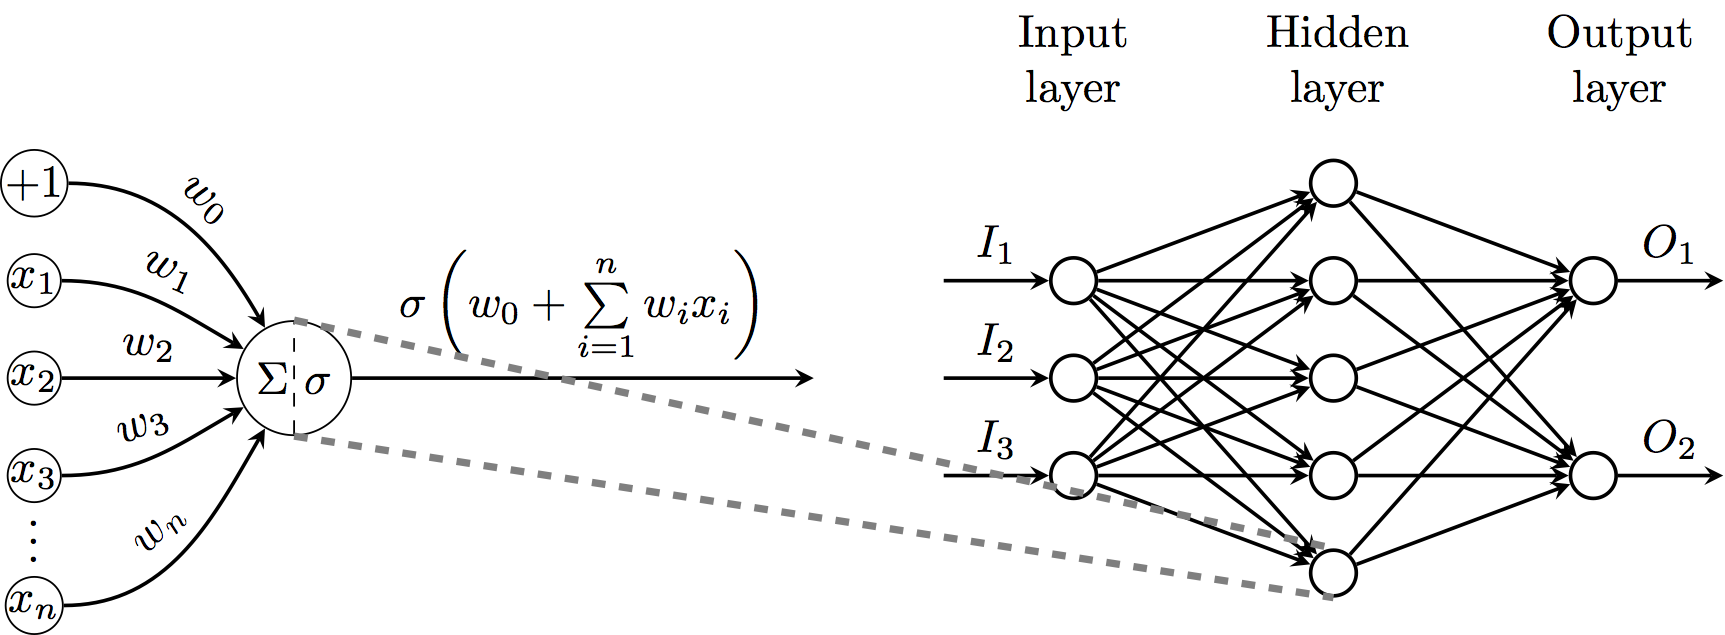
\includegraphics[width=0.95\textwidth]{images/MLP}
	\caption{Multilayer Perceptron (MLP)}
	\label{fig:mlp}
\end{figure}


Bei diesem Netzwerktyp entspricht der Wert eines Knotens einer linearen Überlagerung $n$ sigmoidaler Funktionen, ausgedrückt durch 

\begin{equation} 
\label{eq:feedforward}
\sigma(w_0 + \sum_{i=1}^{n} w_i x_i)
\end{equation}

Die lineare Überlagerung der Netzwerkgewichte $w_1,w_2,...,w_n$ multipliziert mit den Eingangsgrößen $x_1,x_2,...,x_n$ und verschoben um den Wert $w_0$ wird nochmals durch eine Aktivierungsfunktion transformiert. Mögliche Aktivierungsfunktionen sind die \textit{sigmoidale}-Funktion $\sigma(z) = \frac{1}{1 + e^{-z}}$, die \textit{tangenssigmoidale}-Funktion $\phi(z)=\frac{2}{1 + e^{-2z}}-1$ und die \textit{lineare} Funktion $a(z)=z$. \\ 
Die Auswahl der Aktivierungsfunktion ist hierbei vom konkreten Anwendungsfall abhängig. Das Training bzw. die Parametrisierung des Netzes geschieht nun in zwei Schritten. Im ersten Schritt findet eine Übergabe der Eingangsgrößen $x_1,x_2,...,x_n$ an das Netz statt. Weiterhin nehmen die Netzwerkgewichte $w$ anfangs zufällige Werte an. Da die Eingangsgrößen und die Netzwerkgewichte bekannt sind, kann jeder Knotenwert nach Gleichung \ref{eq:feedforward} berechnet werden. Die nachfolgenden Knotenwerte der nächsten Schicht lassen sich somit sukzessive als Funktion der vorherigen Schicht berechnen. Auf diese Weise des Vorwärtsrechnens findet eine Transformation der Eingabegrößen $x_1,x_2,...x_n$ in ein Ausgangssignal $\hat{y}$ statt. \\
Der zweite Schritt umfasst nun die Adaptierung der Netzwerkgewichte, sodass die vom Netz herausgegebenen Ausgabegrößen $\hat{y}$ mit den gemessenen Ausgabegrößen $y_i$ möglichst übereinstimmen. Dabei ist es zweckmäßig, die Abweichung zwischen diesen Größen in Form der Fehlerfunktion 

\begin{equation}
E(w) = (y_i-N(x_i|w))^{2}
\end{equation}

zu beschreiben. Die Adaptierung der Netzwerkgewichte beschränkt sich nun darauf, die Fehlerfunktion zu minimieren. Eine der gängigsten Methoden ist die Methode des Gradientenabstieges. Diese gibt als Adaptionsregel für die Netzwerkgewichte 

\begin{equation}
\label{eq:weight_adapt}
\Delta w_i = \epsilon  (-\nabla E_i) = \epsilon * - \dfrac{\partial E}{\partial w}\bigg|_{w_i}
\end{equation}

mit $\epsilon$ als Lernrate bzw. Adaptionsschrittweite vor. Das Ziel besteht darin, für die Fehlerfunktion $E(w)$ die partiellen Ableitungen $\dfrac{\partial E}{\partial w}\bigg|_{w_i}$ zu identifizieren und gleich null zu setzen. Damit würde die Fehlerfunktion $E(w)$ ein lokales Minima erreichen. Dies geschieht durch die lokale Suche nach dem Minimum der Fehlerfunktion $E(w)$ in Richtung des steilsten Abstiegs. Die Richtung des steilsten Abstiegs entspricht dabei dem negativen Gradienten von $E$ nach den Netzwerkgewichten $w$.\\ 
Die Adaption findet für jedes Datenpaar $((x_1,x_2,...,x_n)|(y_1))$ statt. Durch das Wiederholen des Adaptionsvorgang passt sich das Netz dem zu modellierenden Systemverhalten an. \\

Wie bereits erwähnt, bietet sich die Methode des Gradientenabstieges als ein mögliches Verfahren zur Minimierung der Fehlerfunktion an. Es gibt darüber hinaus in der Literatur eine Vielzahl von Verfahren, die sich in folgende Kategorien einteilen lassen:

\begin{itemize}
	\item Gradientenverfahren erster Ordnung
	\item Gradientenverfahren zweiter Ordnung
	\item stochastische Optimierungsverfahren
	\item Verfahren der globalen Optimierung
\end{itemize}


Den Verfahren der ersten Kategorie ist gemein, dass die Berechnung des Gradienten des Gütefunktionals

\begin{equation}
\nabla E_i = \dfrac{\partial E}{\partial w}\bigg|_{w_i}
\end{equation}

in jeder Iteration problematisch ist, da sich die Gradienten nicht in einem Schritt berechnen lassen. In der Regel kommt für die Lösung dieses Problems der Backpropagation-Algorithmus zum Einsatz. Dieser wendet die Kettenregel an, um die Gradienten in mehrere Faktoren, bestehend aus partiellen Ableitungen, zu zerlegen. Auf diese Weise können die partiellen Ableitungen der letzten Schicht, welche in der Regel bekannt sind, benutzt werden können, um die partiellen Ableitungen der vorangehenden Schichten zu bestimmen. 
Die Ermittlung der partiellen Ableitungen findet also von der letzten bis zur ersten Schicht, also rückwärts, statt. Nach Ermittlung der partiellen Ableitungen aller Schichten, kann die Adaption der Netzwerkgewichte gemäß einer Adaptionsregel, siehe \ref{eq:weight_adapt}, erfolgen. Während des Adaptionsprozesses nimmt der Gesamtfehler ab. Sinkt der Gesamtfehler über alle Netzausgänge $y_1,...,y_m$ unter eine festgelegte Grenze, bricht das Training des Netzes ab. \\

Es bleibt festzuhalten, dass die Anpassungsfähigkeit des Netzes an das nichtlineare Verhalten dynamischer Systeme von folgenden Faktoren abhängt:

\begin{itemize}
	\item Anzahl der Neuronen
	\item Anzahl der Schichten
	\item Wahl des Algorithmus zur Minimierung der Fehlerfunktion
	\item Auswahl der Aktivierungsfunktionen
	\item Repräsentationsfähigkeit der Trainingsdaten
	\item Wahl des Regressors
	
\end{itemize}





\chapter{Ausblick}





% =================================================================================
% Anhang
% =================================================================================
\appendix % Damit wird der Anhang begonnen. Die Kapitel werden ab jetzt mit Buchstaben nummeriert
%\input{inc/Anhang_Messrauschen.tex}
%\input{inc/Anhang_MesstasterHalterung.tex}
%\input{inc/Herleitung_Bauteildynamik.tex}

% =================================================================================




% =================================================================================
% Literaturverzeichnis
% =================================================================================
\cleardoublepage
\phantomsection					% Für Aufnahme ins Inhaltsverzeichnis
\addcontentsline{toc}{chapter}{\bibname}	% In Inhaltsverzeichnis von
											% Dokument und pdf aufnehmen
\bibliographystyle{gerabbrv}	% Festlegen, wie das Verzeichnis und die Verweise
%\bibliographystyle{plain}
								% im Text aussehen
\bibliography{./bib/literature}	% Literaturverzeichnis einfügen, mit Angabe der
%\bibliography{./bib/literature2}	% Literaturverzeichnis einfügen, mit Angabe der
								% Bibtex-Datei
% =================================================================================

\end{document}
